\documentclass[11pt]{article}

\usepackage{times}

\usepackage{epsfig}

\setlength{\topmargin}{-0.5in}
\setlength{\textheight}{9.5in}
\setlength{\oddsidemargin}{0cm}
\setlength{\textwidth}{6.5in}


\newcommand{\bea}{\begin{eqnarray}}
\newcommand{\eea}{\end{eqnarray}}

\newcommand{\dpt}[2]{\frac{\partial #1}{\partial #2}}
\newcommand{\Dpt}[2]{\frac{D #1}{D #2}}
\newcommand{\ov}{\overline}
\newcommand{\LM}[1]{\overline{#1}^L}

\newcommand{\bfx}{{\bf x}}

\newcommand{\be}{\begin{equation}}
\newcommand{\ee}{\end{equation}}

\pagestyle{empty}


\begin{document}

\section*{5.5 Hydrodynamic and Wave Modeling (NEARCOM)}

The Nearshore Community Model (NEARCOM) is an extensible, user-configurable model system for nearshore wave, circulation and sediment processes developed during the National Oceanographic Partnership Program (NOPP). The model consists of a “backbone”; the master program, handling data input and output as well as internal storage, together with a suite of modules, each of which handles a focused subset of the physical processes being studied. A total of 10 modules exists, developed by a large group of researchers from various institutions. Example modules are: 1) A wave module simulates wave transformation over arbitrary coastal bathymetry and predicts radiation stresses and wave-induced mass fluxes; 2) A circulation module simulates the slowly varying current field driven by waves, wind and buoyancy forcing, and provides information on the bottom boundary layer structure; and 3) A seabed module simulates sediment transport, determines the bedform geometry, parameterizes the bedform effect on bottom friction, and computes morphological evolution resulting from spatial variations in local sediment transport rates.

\begin{figure}[h!]
\centering
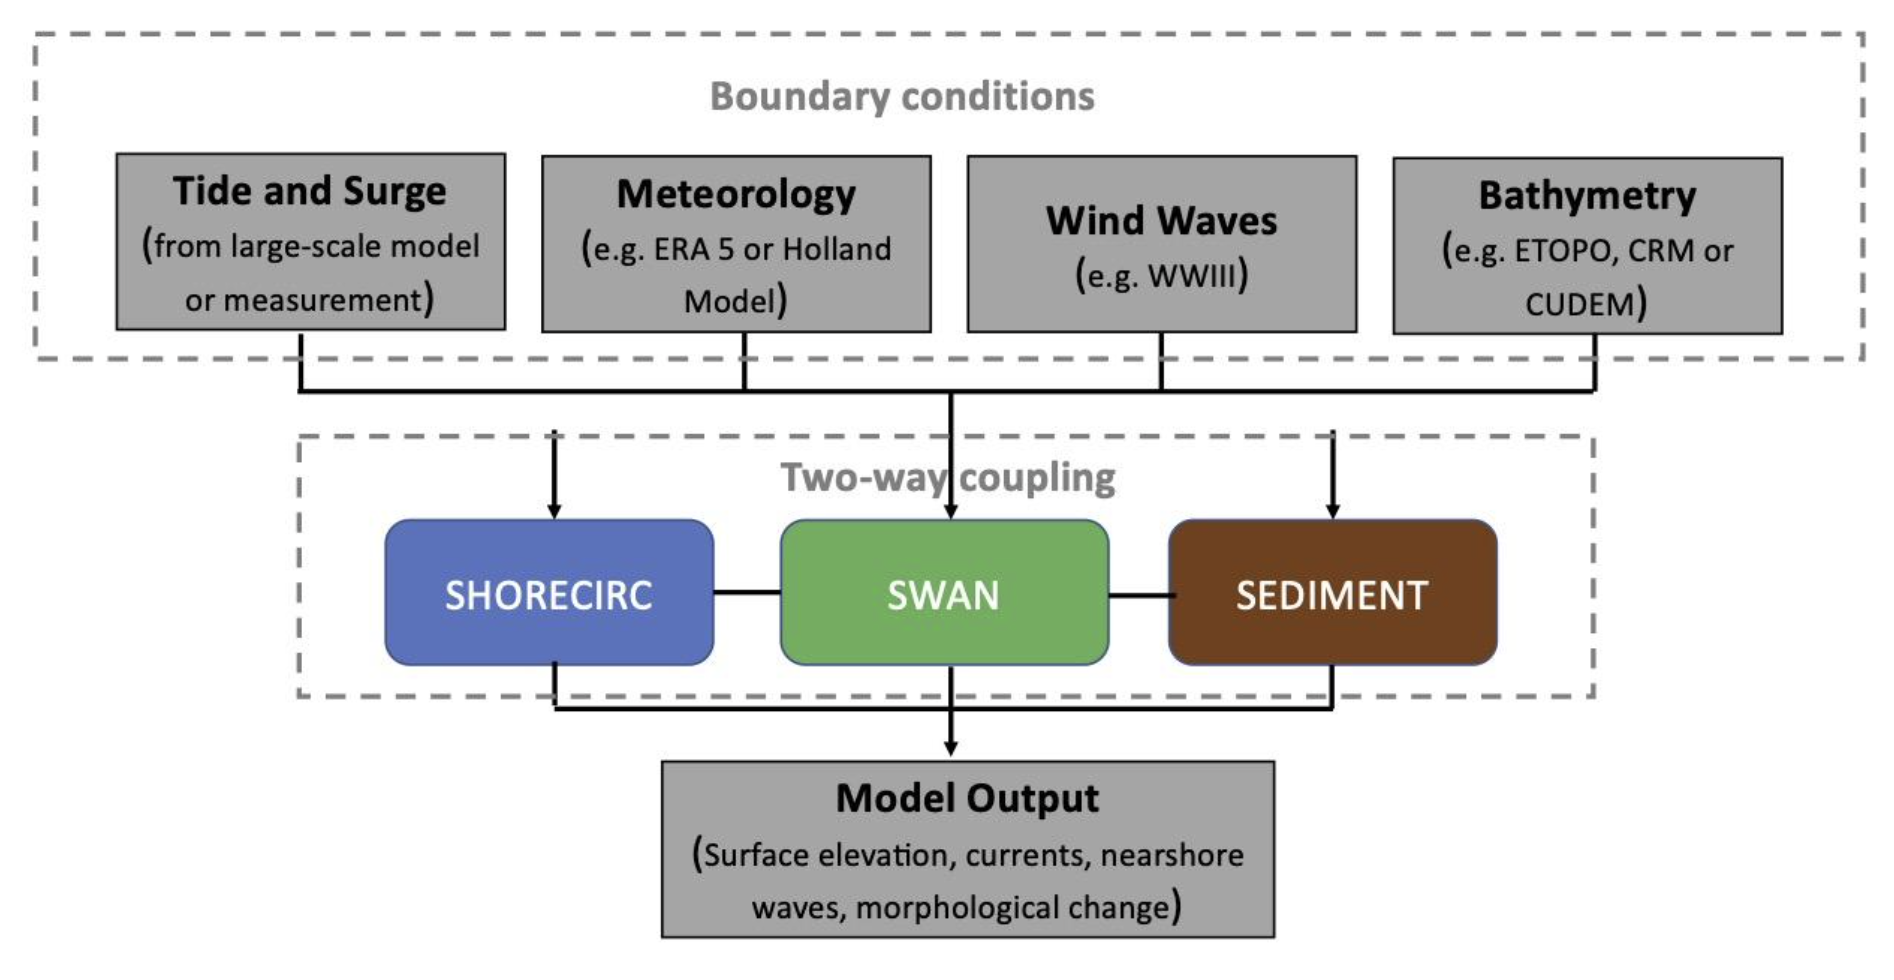
\includegraphics[width=\textwidth]{./figures/nearcom_chart.png}
\caption{The model coupling framework in NEARCOM-TVD. }
\label{nearcom_chart}
\centering
\end{figure}

\subsection*{5.5.1 Selection of wave and circulation modules in NEARCOM}

\begin{figure}[h!]
\centering
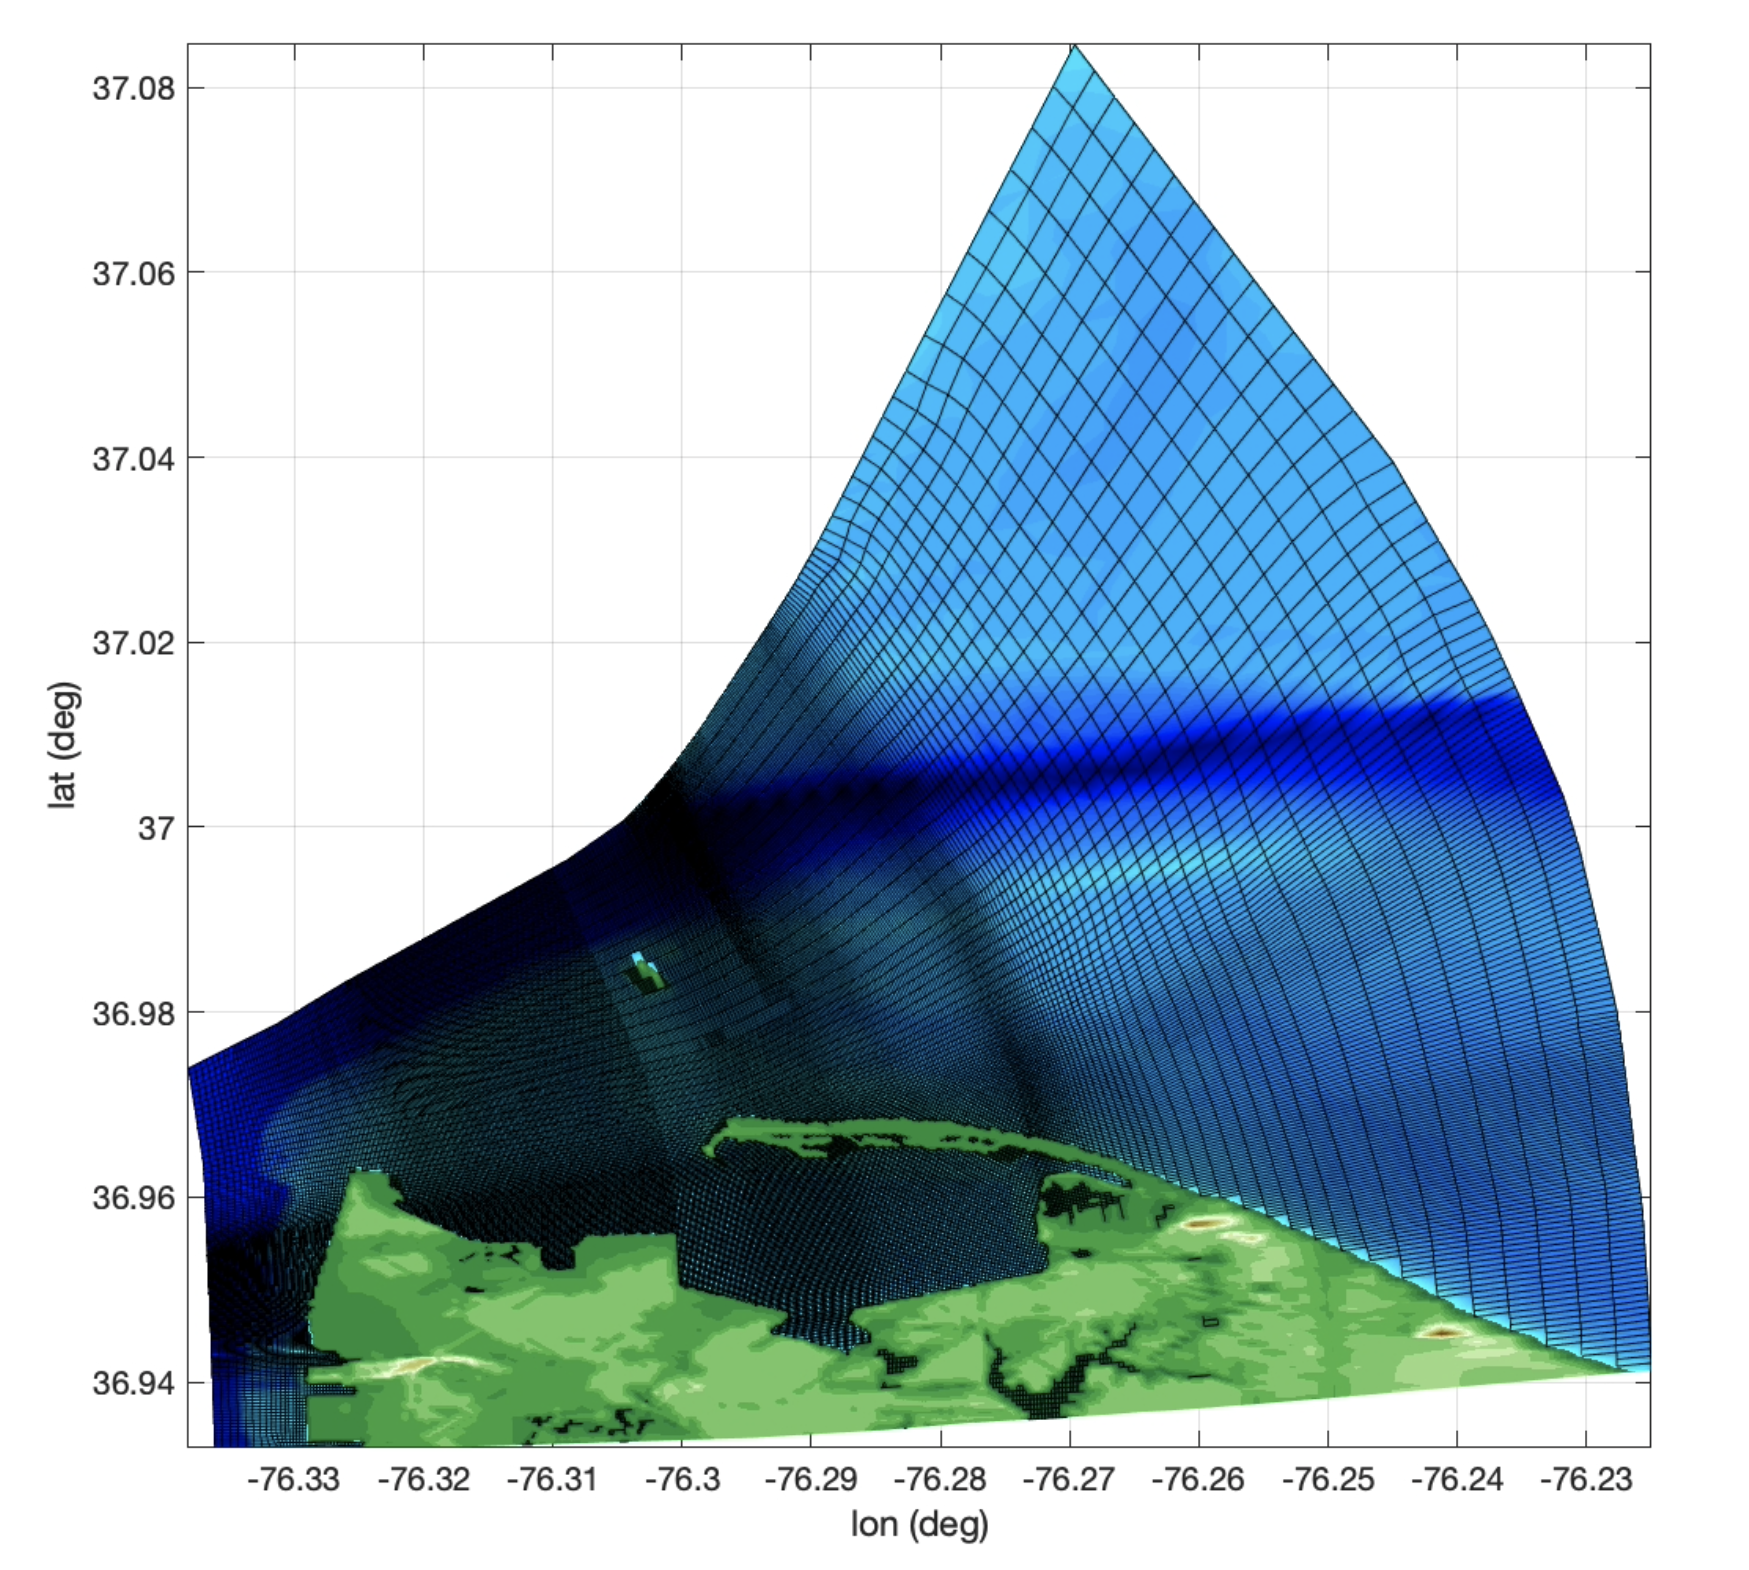
\includegraphics[width=\textwidth]{./figures/nearcom_grid.png}
\caption{Computational grid of NEARCOM. The bathymetry is indicated by colors. The maximum grid size is 200 m offshore and the minimum grid size is 8 m concentrating at Willoughby Bay and NSN area.}
\label{nearcom_grid}
\centering
\end{figure}

In this demonstration study, we applied the combination of the wave model SWAN and the nearshore circulation model SHORECIRC. The coupled SWAN-SHORECIRC model is also called NEARCOM-TVD, which was developed using a hybrid finite-difference finite-volume TVD-type scheme on a generalized curvilinear grid. SWAN and SHORECIRC are tightly coupled using the coupler, MASTER Program in the MPI-based parallel computing framework. SWAN calculates wind waves and provides SHORECIRC with radiation stresses to get wave setups and nearshore circulation. The current effects on waves are computed in SWAN with the current input from SHORECIRC. The model coupling framework is illustrated in Figure \ref{nearcom_chart}. Note that the sediment transport module was not applied in the demonstration.

\subsection*{5.5.2 NEARCOM setup}

Figure \ref{nearcom_grid} shows the generalized curvilinear grid with the fine grid resolution at Naval Station Norfolk. The highest grid resolution is located at the Willoughby Split coast and Willoughby Bay with the smallest grid cell of 6.78 x 8.12 m. NEARCOM addresses the nearshore processes only and thus the computational domain is smaller than that used for D-Flow FM or ADCIRC in a typical tide-surge simulation. The tidal and surge boundary conditions for NEARCOM are provided by a large-scale model, such as D-Flow FM or ADCIRC. The data format for the boundary conditions is (time, elevation, $<$velocity$>$), where $<$velocity$>$ represents depth-averaged current velocity components and are optional.
The original Holland model (Holland, 1980) was implemented in NEARCOM to model wind/pressure forcing in storm surge simulations. The model also has an optional wind/pressure input which can come from large-scale models. In most NEARCOM applications for storm events, the wind/pressure data are provided by a large-scale model, consistent with the boundary conditions from the same large-scale model.

\section*{5.6 Wave modeling (FUNWAVE-TVD)}
FUNWAVE–TVD is the TVD version of the fully nonlinear Boussinesq wave model (FUNWAVE) developed at the University of Delaware (Shi et al., 2012). It is a public domain model maintained by a group of institutions, including the Center for Applied Coastal Research (CACR) at the University of Delaware, Coastal Hydraulics Laboratory, USACE, and the University of Rhode Island. The FUNWAVE model was initially developed by (Kirby et al., 1998) based on (Wei et al., 1995). The development of the TVD version was motivated by a growing demand for phase- resolving modeling of nearshore waves and coastal inundation during storm or tsunami events and predicting sediment transport and short-term morphological processes in a wave-resolving manner.

As a nearshore shallow-to-intermediate water Boussinesq-type numerical wave model, FUNWAVE can resolve many coastal processes. Related to the scopes of this demonstration project, it can predict wave propagation/transformation, refraction, diffraction, reflection, nonlinear shoaling, wave-induced nearshore circulation, nonlinear wave-wave interaction, wave-current interaction, wave breaking, runup and overtopping, IG waves, nearshore sediment transport, and short-term morphological changes. The TVD-type solver particularly has an advantage in resolving wetting and drying processes accurately in modeling storm-induced coastal inundation. FUNWAVE-TVD has been benchmarked for wind wave application in a series of USACE-funded projects, and tsunami application during the National Tsunami Hazard Mitigation Program (NTHMP) which provided the benchmarking standard for judging model acceptance for use in the development of coastal inundation maps and evacuation plans. Source code, documentation, descriptions, and input files for carrying out benchmark tests and various example calculations are available at the FUNWAVE-TVD site (https://fengyanshi.github.io/build/html/index.html). In this study, FUNWAVE is used to simulate the contribution of wave runup to coastal flooding under hurricane force.

\subsection*{5.6.1 Application of FUNWAVE-TVD modules} 
FUNWAVE-TVD consists of several numerical modules for various applications, including Central Module, Tide Module, Meteo. Module, Sediment Transport Module, Precipitation Module, Subgrid Module, Ship-wake Module, Lagrangian Tracking Module, and Bubble and Foam Module. For the application in this study, the model was used to simulate the total water level and coastal inundation by focusing on the effects of wave-resolving processes, such as wave runup, wave overwash and overtopping in a nearshore shallow water domain. The Central Module and Tide Module are the primary modules used in this application. Tides and storm surges were treated as boundary conditions in the model input. The Tide Module was used for the boundary condition input. Wind forcing is not considered due to the small size of the computational domain.

\subsection*{FUNWAVE-TVD configuration}
Figure \ref{funwave_grid} shows the computational grid in a 2D domain. The model domain spanned 5.8 x 4.4 km and was discretized using a constant 0.75 m x 0.75 m grid spacing. A high resolution (3m DEM) topo-bathymetric dataset was obtained for the area using the NOAA Digital Coast: Data Access Viewer to capture the nearshore beach and dune features for accurate wave runup estimates.  Waves and storm tides (tide + surge) are forced at the open boundary. The wave information was obtained from SWAN simulations, and storm tides were from D-Flow simulations.

\begin{figure}[h!]
\centering
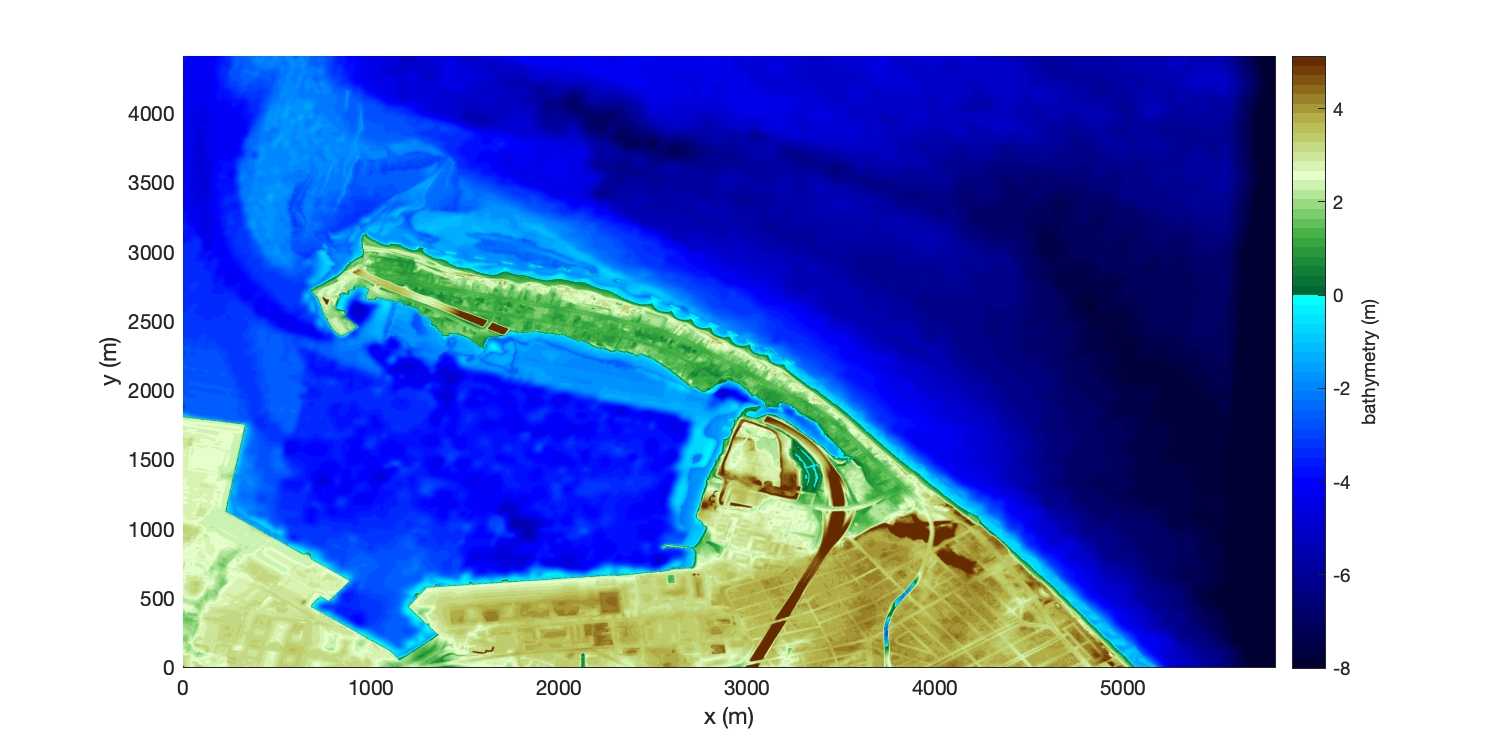
\includegraphics[width=\textwidth]{./figures/funwave_grid_sm.jpg}
\caption{FUNWAVE model grid.}
\label{funwave_grid}
\centering
\end{figure}

\subsection* {3.2.1}

7. Compare the full physics model (class III) to D-Flow FM (class II)

The full physics model provides detailed wind wave information beyond the wave-averaged surface elevation and wave-induced currents. In this demonstration study, FUNWAVE-TVD was applied embedded in the NSN domain of D-Flow FM, concentrating on the wind waves and wave-induced processes along the coast of Willoughby Split. Because of the high computational costs for such a phase-resolving wave model, we selected  six scenarios from the Hurricane Irene-based forcing conditions as described in the NEARCOM section. 

In contrast to the results from D-Flow FM, FUNWAVE-TVD predicted wave-induced setup, runup, and nearshore circulations along the Willoughby Split coast. Wind waves are primarily generated locally during Hurricane Irene, led to small wave setup and runup, with a magnitude of 0.1 m along the coast. The impact of wave setup on the total water level inside Willoughby Bay remains limited. Considering that NSN does not face the open ocean, the wave effects on coastal inundation are minimal.  

\section*{3.x Class II model, NEARCOM}

NEARCOM is a Class II model, similar to D-Flow FM and ADCIRC. Due to the specific inland characteristics of NSN, D-Flow FM and ADCIRC are employed as large-scale/regional-scale models, with the maximum grid resolution unable to resolve the surfzone. Therefore, we utilized the quasi-3D model, NEARCOM, which serves as a nearshore wave-averaged model, specifically focusing on the effects of wave-induced processes on the total water prediction. 

1. Time required to generate computational grid and open boundary conditions

NEARCOM used a structured curvilinear grid based on the Cartesian coordinate. Since the generalized curvilinear grids can be non-orthogonal, they can be generated using either an orthogonal grid generator or a general grid generator. In this study, we used CoastGrid, a MATLAB-based tool with a user-friendly GUI, developed by the University of Delaware. The grid generation process typically takes 1-2 days, depending on modeling experience. 

The open boundary conditions are generated by a time-series of surface elevation and wave spectra or wave bulk parameters at the open boundary locations as provided by the large-scale model, D-Flow FM and SWAN. A MATLAB or FORTRAN-based script can read the time-series and generate what we refer to as 'nesting files' for use in NEARCOM. The entire process, including script execution, result verifiction and test runs may take a day's work for an experienced user. 

2. Time required to conduct a simulation 

With the highest grid resolution of $6.78 \times 8.12$ m, NEARCOM regures more computational time than the large-scale models used in the study. The model can be run on a standard PC with multiple cores or a HPC system. In this study,  the simulations were performed on the community cluster, known as the Caviness distributed-memory Linux System, utilizing 64 cores for each case. Each simulation took approximately 5 hours of wall time. 

 3. Selection of scenarios and simulation time

NEARCOM was used to simulate nearshore processes and estimate the impact of wind waves on total water levels during storms. For this demonstration, we selected six scenarios: two base scenarios corresponding to Hurricane Irene with the ERA and Holland forcing, along with four cases featuring varying forcing parameters. These parameters indicated the extremely large surge conditions in the D-Flow FM model. The six scenarios are listed in table X. 

The simulation time period is relatively shorter than that performed in D-Flow FM.  We selected the time period is from 27-Aug-2011 6:00 to 28-Aug-2011 6:00. During this interval, both the storm tide and wave height reach their maximum in all six scenarios.   

4. Model capability in predicting wave-induced processes

Compared to the large-scale models, D-Flow FM and ADCIRC, NEARCOM provided results of wind waves and wave-induced setup and currents during a storm. The model predicted  the wave height distribution consistent with the Class III model, FUNWAVE-TVD (as discussed in the next section), but with a smoother distribution. Wind waves are generated locally during Hurricane Irene and do not penetrate into the bay. Among the six scenarios, the largest wave height can be found in Scenario SLR = 1.3 m due to larger waves at the open boundary. 
 
 The model results reveal wave setup along the coast of Willoughby Split in all six scenarios. The magnitude of wave setup is 0.1 m, approximately 10 \% of the significant wave height, consistent with the predictions based on the theory of radiation stresses (Longuet-Higins and Steward, 1962). This small wave setup does not lead to additional inundation in the back bay areas as evidenced by the comparison of cases with and without waves. The model results from the six scenarios demonstrate strong alongshore currents generated by wind waves along the coast of Willoughby Split. Notably, currents reversals occur during the surge receding stage when wave-induced currents and receding currents point in different directions.  Comparing cases with and without waves indicates that  the wave-induced currents are significant larger than tide- and surge-induced currents, potentially contributing to coastal erosions. 

5. Model capability in predicting coastal inundation

Because NEARCOM simulations primarily focus on nearshore processes, the flood area estimations include Willoughby Split which lies outside of NSN. However, these estimations can help assess whether wave-induced processes affect storm inundation in NSN. 
 
 The NEARCOM results indicate that the flooded areas in the selected scenarios primarily distributed at Willoughby Split, except for the scenario with SLR = 1.3 m, which suggests significant inland flooding. The flooded areas (within the computational domain) from the six scenarios are listed in table X
 
 \begin{table}[h!]
 \caption{Scenarios modeled by NEARCOM and flooded area}
 \centering
 \begin{tabular}[t]{c c c  c} \hline
  Scenario & Time of Peak Storm Tide  &  Peak Elevation (m)  &  flooded area (km$^2$ )    \\ \hline
  ERA5      & 27-Aug-2011 23:00  & 1.55   & 1.41  \\
  HM      & 28-Aug-2011 00:00  & 1.76   & 1.85 \\
  Acc GN 1m      & 28-Aug-2011 00:00  & 1.75   & 1.85  \\
  RMW F1.25      & 28-Aug-2011 00:00  & 1.66   & 1.80  \\
   SLR 1.3m      & 28-Aug-2011 00:00  & 3.02   & 6.98  \\
    WSF 1.225     & 27-Aug-2011 23:00  & 2.45   & 3.97  \\
     \hline
 \end{tabular}
% \vskip 0.2cm
\end{table}
 


\section*{3.3 Class III model, FUNWAVE-TVD}

1. Time required to generate computational grid and open boundary conditions

The Cartesian mode of FUNWAVE-TVD uses a rectangular grid, which can be generated directly from a DEM without the need for additional grid generation software. To prevent wave reflection and diffraction at lateral boundaries, it is essential to generate a grid with a periodically (cyclically) bathymetric condition by extending the model domain. Typically, the grid generation process takes 1-2 hours depending on the modeler's experience. 

The open boundary conditions, including wave conditions and storm-tide elevations, are set up in the input file. The process is straightforward:  given wave spectra by the large domain model SWAN and surface elevation by D-Flow FM. 


2. Time required to conduct a simulation 

 The full physics model is computationally expensive due to its higher grid resolution and wave phase-resolving capabilities compared to the wave-averaged model (class II). Typically, it is performed on a HPC system with a large number of computing cores in an MPI-based operation. In this study, simulations were conducted on the HPE Cray EX4000 system, utilizing 2304 cores for each case. Each simulation took approximately 2.5 hours of wall time. 

3. Selection of scenarios

The same as the NEARCOM model, we selected six scenarios: two base scenarios of Hurricane Irene (ERA  and Holland), and four cases with different forcing parameters. These cases indicated extremely large surge conditions in the D-Flow FM model.  

4. Model capability in predicting wind waves and wave-induced processes

The full physics model provides detailed wind wave information with a phase-resolved fashion.  It predicts wave propagations and transformations, including wave refraction, diffraction, reflections from beaches and coastal structures, wave-wave interaction. The model results include wave-induced currents, wave setup, runup, wave overtopping, and overwash. Wave-current interaction is taken into account with fully resolved physics, especially for phase-coupled mechanisms, such as wave refraction by currents and waves in a transient rip/alongshore system. 

The model predicted nearshore waves with wave heights consistent with those from the NEARCOM scenarios. The spatial distributions of wave height show apparent stripe patterns, which are induced by wave-coherence, in contrast to the smooth distributions from NEARCOM. In the scenario with SLR = 1.3m, wave height increased by 35\% compared to the base scenario using ERA5 forcing. This represents the largest wave height among the six scenarios.

The model results provide distributions of wave setup along the Willoughby Split coast. The magnitude of wave setup is 0.1 m, consistent with the NEARCOM predictions. The small wave setup does not induce any additional coastal flooding.  

Wave-induced currents are generated in the surfzone along the Willoughby Split coast. Eddies associated with the wave dissipation are distributed along the coast, as well as inside Willoughby Bay as the Willoughby Split is flooded in the case of SLR = 1.3 m. 

5. Model capability in predicting coastal inundation
 
The flooded areas were calculated within the computational domain in the six scenarios. Different from D-Flow FM which does not provided a flooding estimate in Willoughby Split due to a lower grid resolution, FUNWAVE-TVD predicted detailed flooded areas in the entire computational domain, including Willoughby Split. The results from the two base scenarios of  Hurricane Irene are comparable to the STORM anecdotal data (Figure 31). 


\section*{6.5 NEARCOM} 

\begin{figure}[h!]
\centering
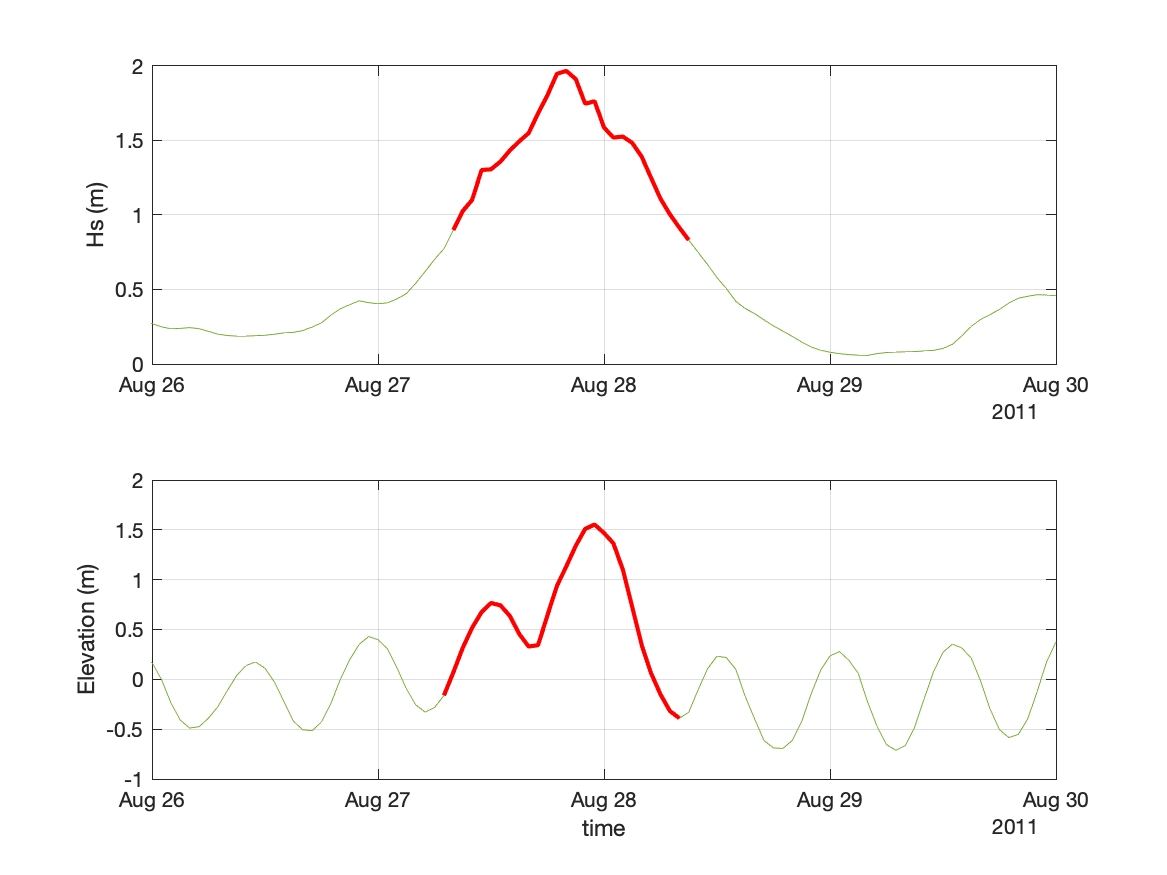
\includegraphics[width=\textwidth]{./figures/nearcom_wave_flow.jpg}
\caption{NEARCOM model input boundary conditions. Time series of significant wave height (top) and surface elevation (bottom) at the boundary point of (36.9742N, 76.2271W). The simulation period is indicated by the red lines. }
\label{ERA5_time}
\centering
\end{figure}

\subsection*{6.5.1 Results of waves, storm tide, and nearshore circulation, Scenario ERA5, for example}

NEARCOM predicts nearshore waves, storm tide, wave setup and wave-induced currents. Wave-current interaction is taken into account through the tight coupling of the wave module and circulation module.  To demonstrate the results from the coupled model, we illustrate the results of waves, surface elevation, and current fields at three snapshots, the beginning stage, peak and receding stage of the storm tide from Scenario ERA5. 

Figure \ref{ERA5_hs_1} shows the distribution of wave height (color) and wave direction (vector) at 27-Aug-2011 17:00, the beginning of the storm tide. Waves concentrate on the open coast. The obliquely incident waves generate strong alongshore currents as shown in Figure \ref{ERA5_eta_1}.

 At  27-Aug-2011 23:00, both the storm tide and wave height reach the peak. The surfzone become wider compared to that at the lower storm tide as shown in Figure \ref{ERA5_hs_2}. The alongshore currents extend to the tip of Willoughby Spit and inside Willoughby Bay (Figure \ref{ERA5_eta_2}). Willoughby Split is partially flooded on both the beach side and the back bay side. 
 
 During the receding period, both the wave height (Figure \ref{ERA5_hs_3}) and the storm tide (Figure \ref{ERA5_eta_3}) decrease. Most of flooded regions drain, leaving small ponding areas at Willoughby Spit.   

\begin{figure}[h!]
\centering
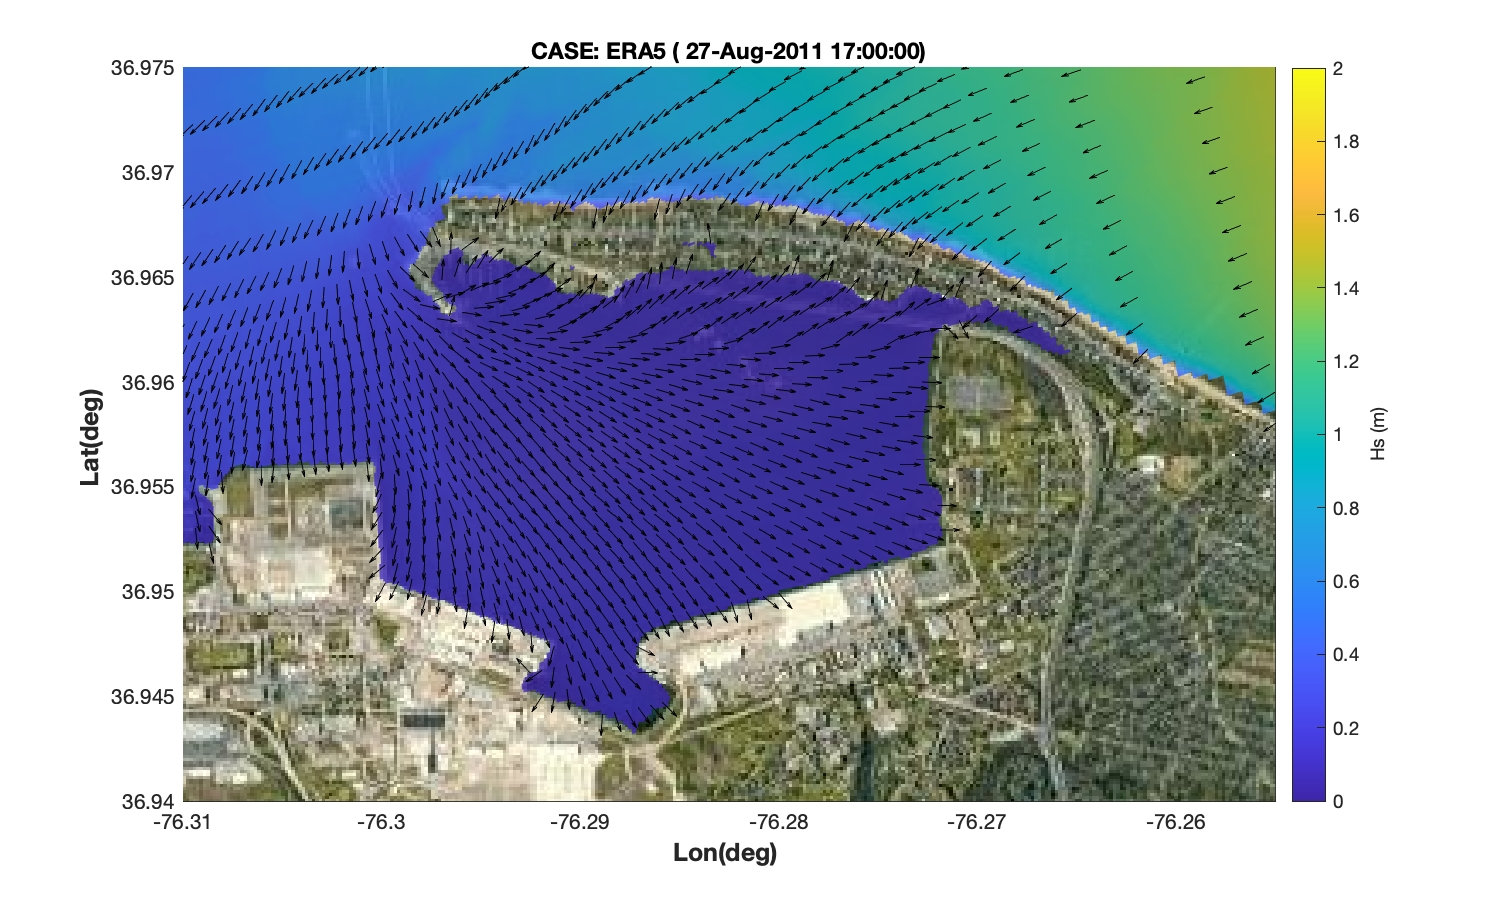
\includegraphics[width=\textwidth]{./figures/nearcom_hs_ERA5_55.jpg}
\caption{Snapshot of wave height distribution (color) and and wave direction (vectors) at the beginning of the storm tide (27-Aug-2011 17:00) for scenario ERA5.}
\label{ERA5_hs_1}
\centering
\end{figure}

\begin{figure}[h!]
\centering
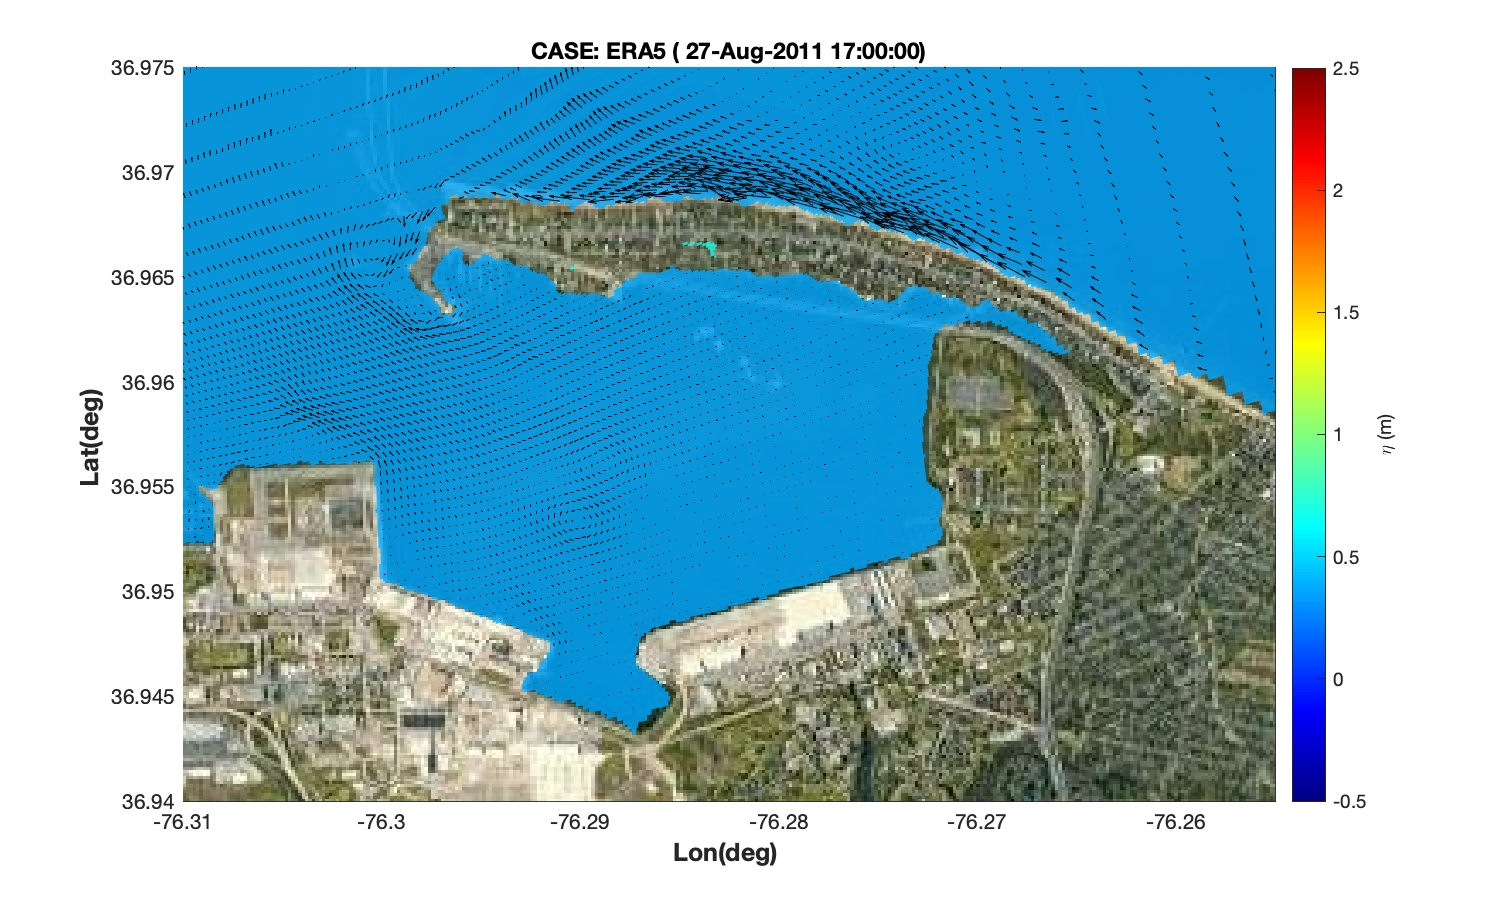
\includegraphics[width=\textwidth]{./figures/nearcom_ele_ERA5_55.jpg}
\caption{Snapshot of surface elevation (color) and and currents (vectors) at the beginning of the storm tide (27-Aug-2011 17:00) for scenario ERA5.}
\label{ERA5_eta_1}
\centering
\end{figure}

\begin{figure}[h!]
\centering
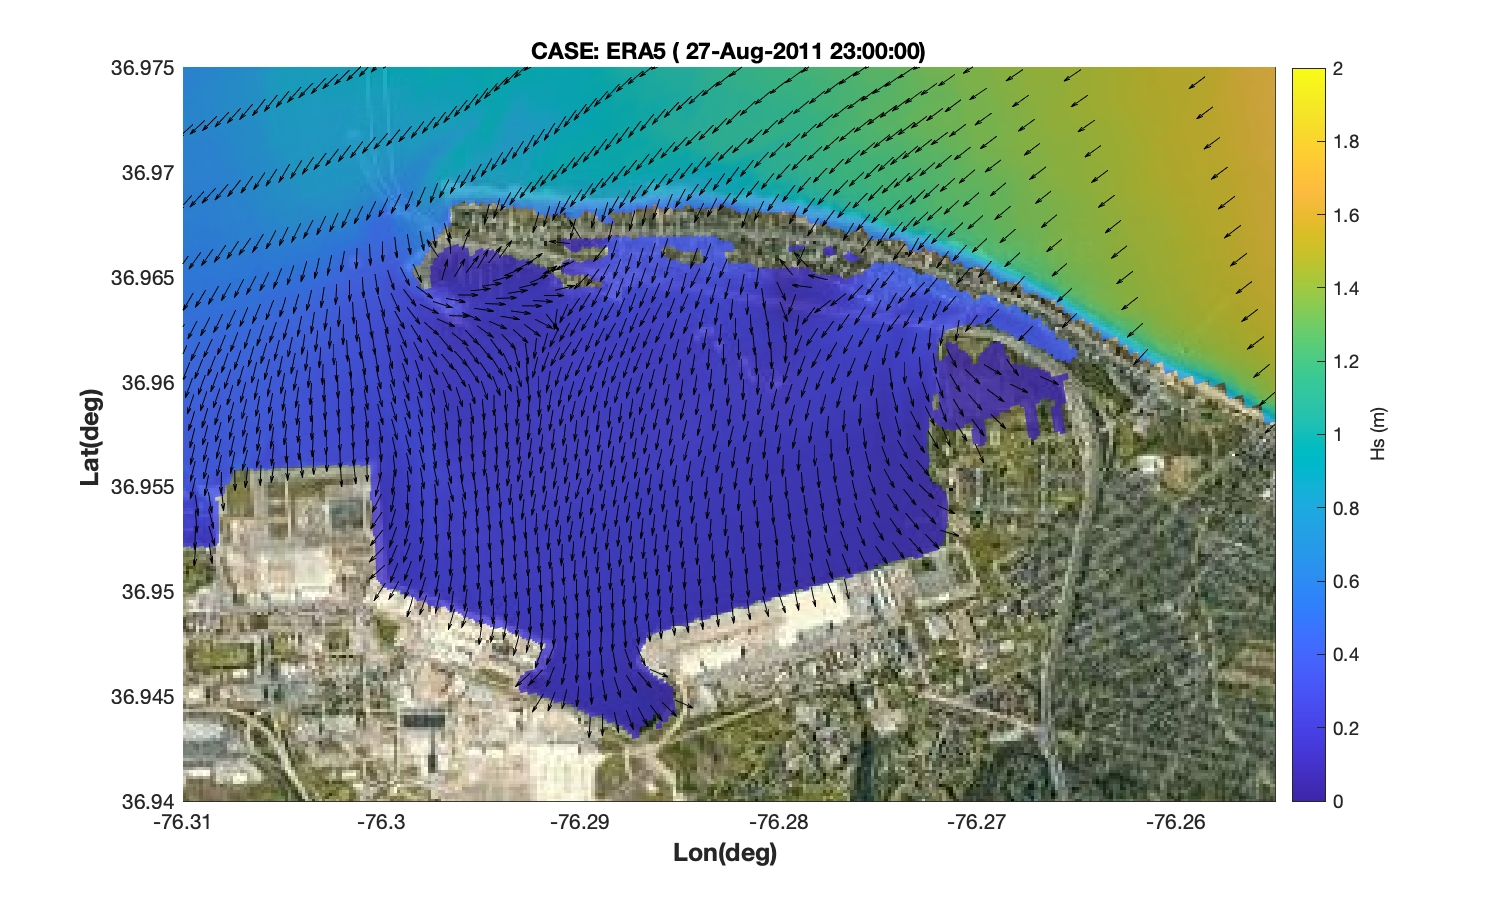
\includegraphics[width=\textwidth]{./figures/nearcom_hs_ERA5_91.jpg}
\caption{Snapshot of wave height distribution (color) and and wave direction (vectors) at the peak of the storm tide (27-Aug-2011 23:00) for scenario ERA5. }
\label{ERA5_hs_2}
\centering
\end{figure}

\begin{figure}[h!]
\centering
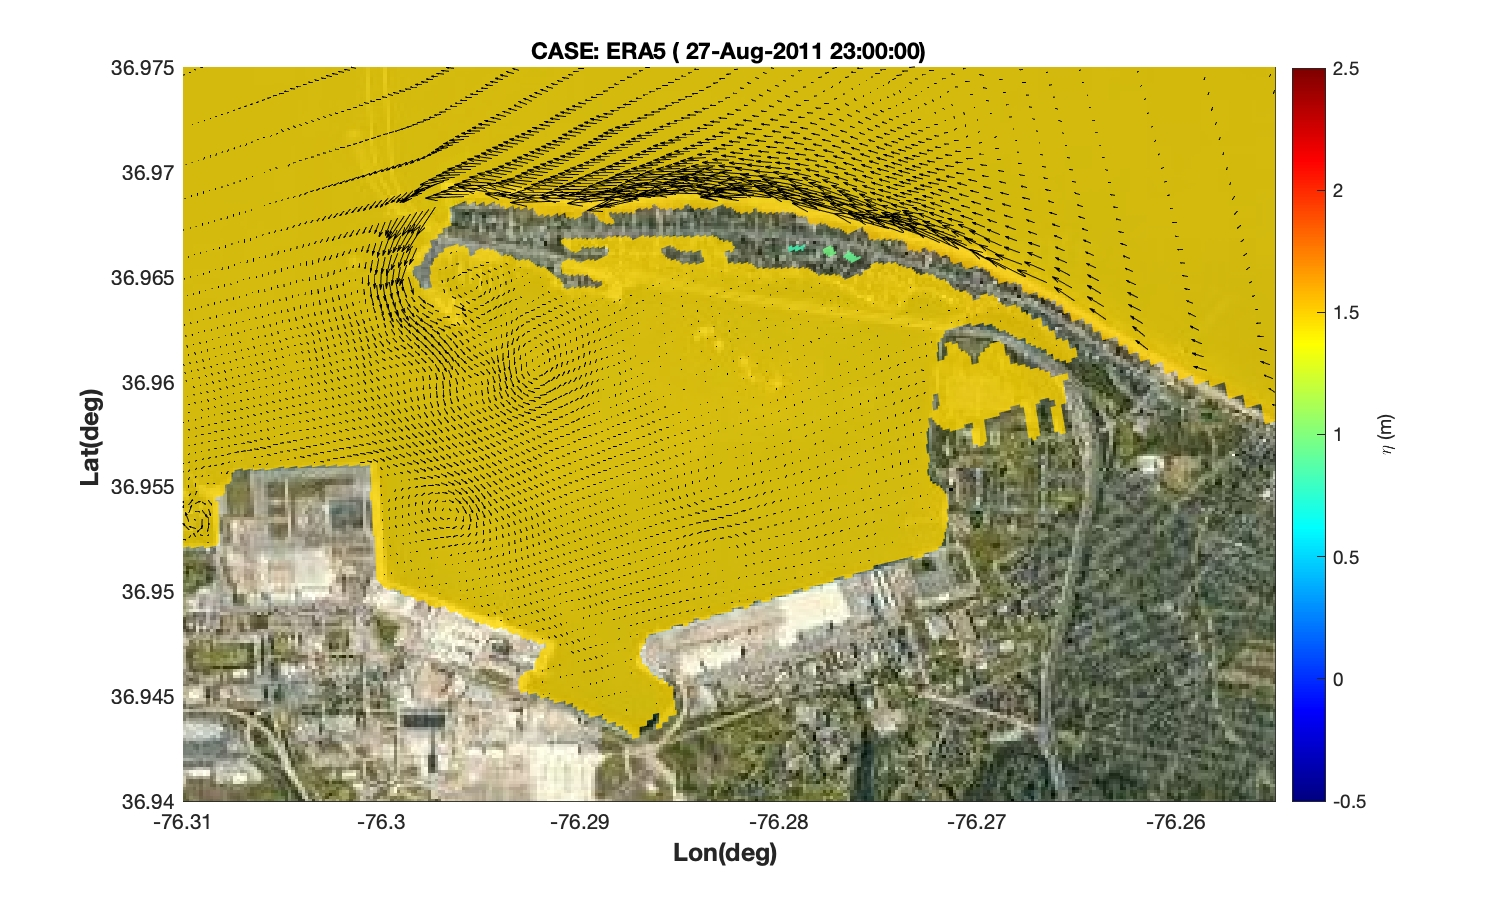
\includegraphics[width=\textwidth]{./figures/nearcom_ele_ERA5_91.jpg}
\caption{Snapshot of surface elevation (color) and and currents (vectors) at the peak of the storm tide (27-Aug-2011 23:00) for scenario ERA5.}
\label{ERA5_eta_2}
\centering
\end{figure}

\begin{figure}[h!]
\centering
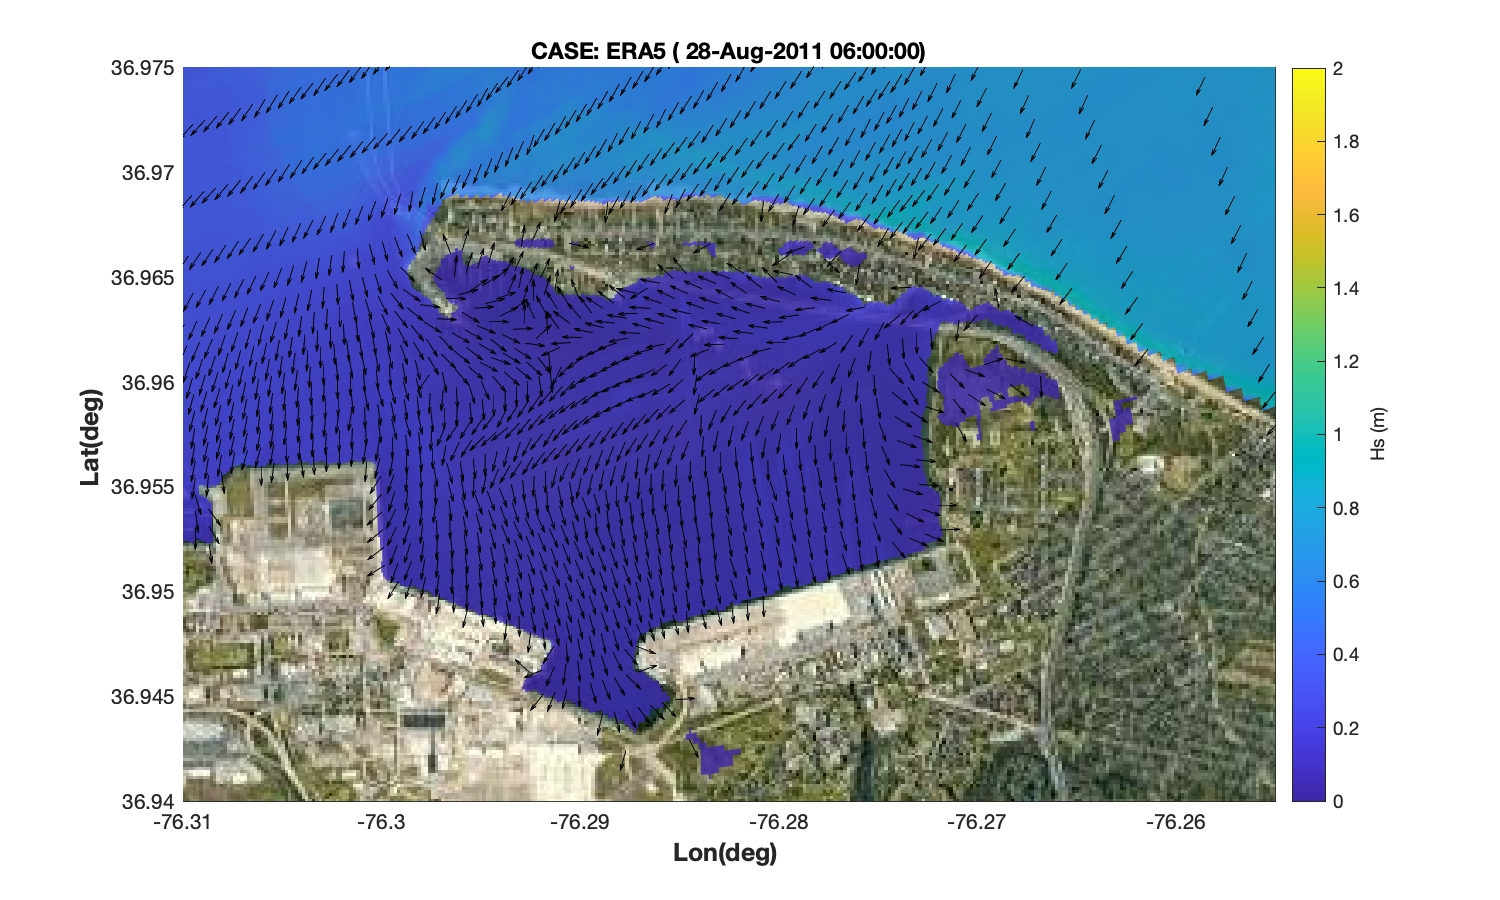
\includegraphics[width=\textwidth]{./figures/nearcom_hs_ERA5_133.jpg}
\caption{Snapshot of wave height distribution (color) and and wave direction (vectors) at the receding stage (28-Aug-2011 06:00) for scenario ERA5. }
\label{ERA5_hs_3}
\centering
\end{figure}

\begin{figure}[h!]
\centering
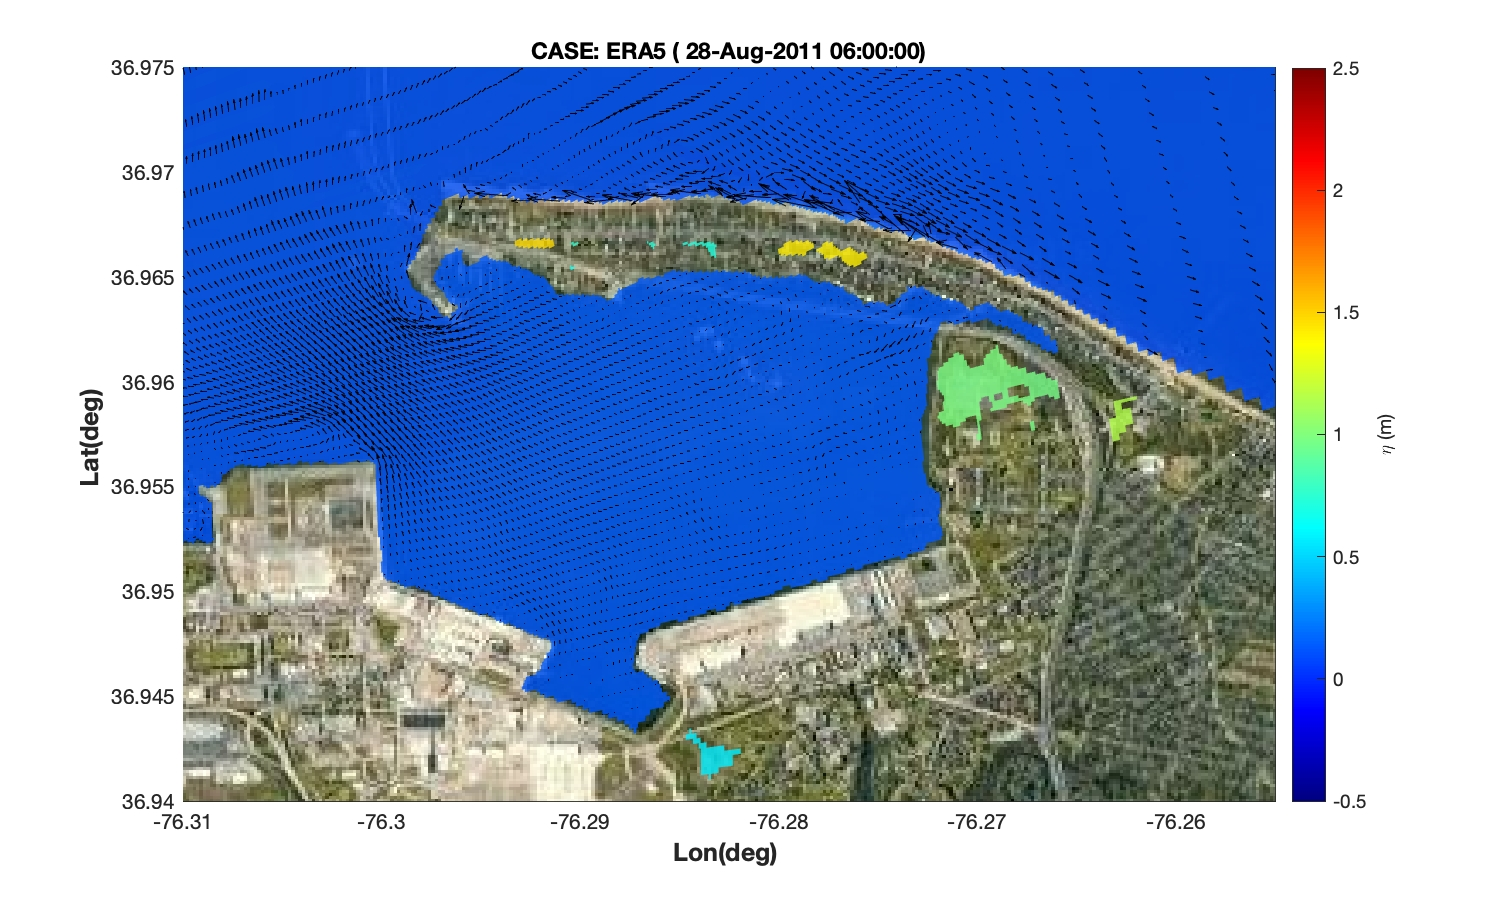
\includegraphics[width=\textwidth]{./figures/nearcom_ele_ERA5_133.jpg}
\caption{Snapshot of surface elevation (color) and and currents (vectors)  at the receding stage(28-Aug-2011 06:00) for scenario ERA5. }
\label{ERA5_eta_3}
\centering
\end{figure}

% wave versus no wave
\subsection*{6.5.3 Wave-induced processes, Scenario ERA5, for example}

One of the objectives in this study is to examine the contribution of wind waves to the total water level during storms. In the NSN domain, wind waves are generated locally during storm events, resulting in a fetch-limited generation mechanism. NSN is not significantly exposed to large waves. As a result, wave setup is expected to be negligible compared to the wind-induced surge. To illustrate the effects of wave-induced setup and currents, we conducted an additional run for Scenario ERA5 without coupling the wave model SWAN.

 Figure \ref{ERA5_eta_wo_wave} shows a comparison of surface elevation and currents between the cases with and without wave contribution at the peak storm tide (27-Aug-2011 23:00). The wave setup is evident in the surface elevation comparison (top panel versus bottom panel), with approximately 0.1 meters distributed in the surfzone along the coast. In addition, wave-induced currents are much stronger than the wind-induced currents. Although the water level within Willoughby Bay is also affected by wave setup at the beach near the bay mouth, the slight increase in surface elevation does not lead to additional flooding inside the bay. 

\begin{figure}[h!]
\centering
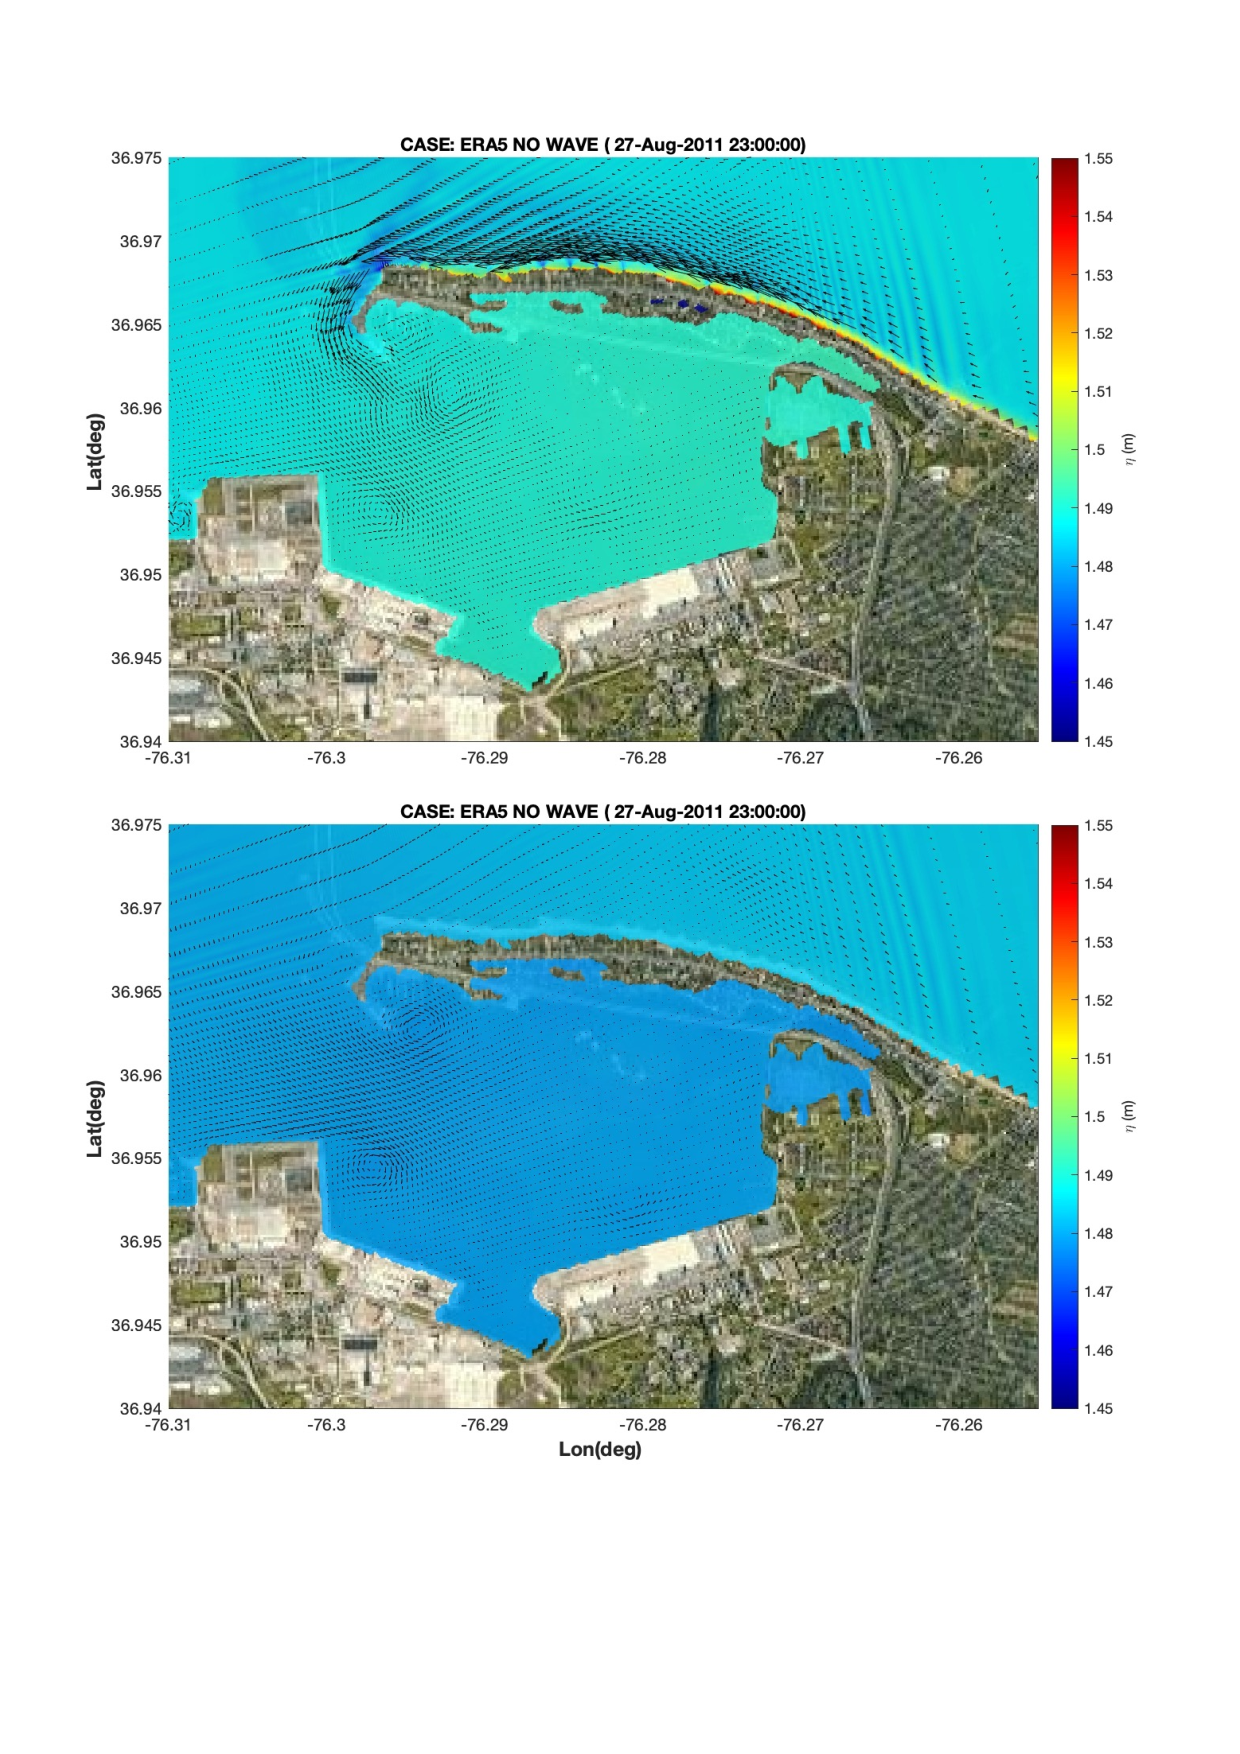
\includegraphics[width=\textwidth]{./figures/nearcom_wo_wave.pdf}
\caption{Comparison of surface elevation and currents at the peak storm tide between models with and without the wave module coupled in the NEARCOM system.}
\label{ERA5_eta_wo_wave}
\centering
\end{figure}

% 6 cases
\subsection*{6.5.4 Comparisons between six scenarios}
Figure \ref{nearcom_6_cases_hs} illustrates the wave height distribution at the peak of storm tide from all six scenarios. In each scenario, wave height decreases from east to west outside the bay. Inside the bay, the waves are small. However, for Scenarios SLR 1.3m and WSF 1.225, waves penetrate inside the bay due to submergence of  Willoughby Spilt. 

The surface elevation and currents at the peak of storm tide are compared in Figure \ref{nearcom_6_cases_eta}. As expected, the largest surface elevation appears in Scenario SLR 1.3m. Large currents can be found inside the bay, that attributes to the overwash at Willoughby Split. For other cases, strong current appear alongshore and at the bay mouth. 

Figure \ref{nearcom_6_cases_flood} shows the flooded areas from all six cases. The results are compared in Figure \ref{nearcom_bars}

\begin{figure}[h!]
\centering
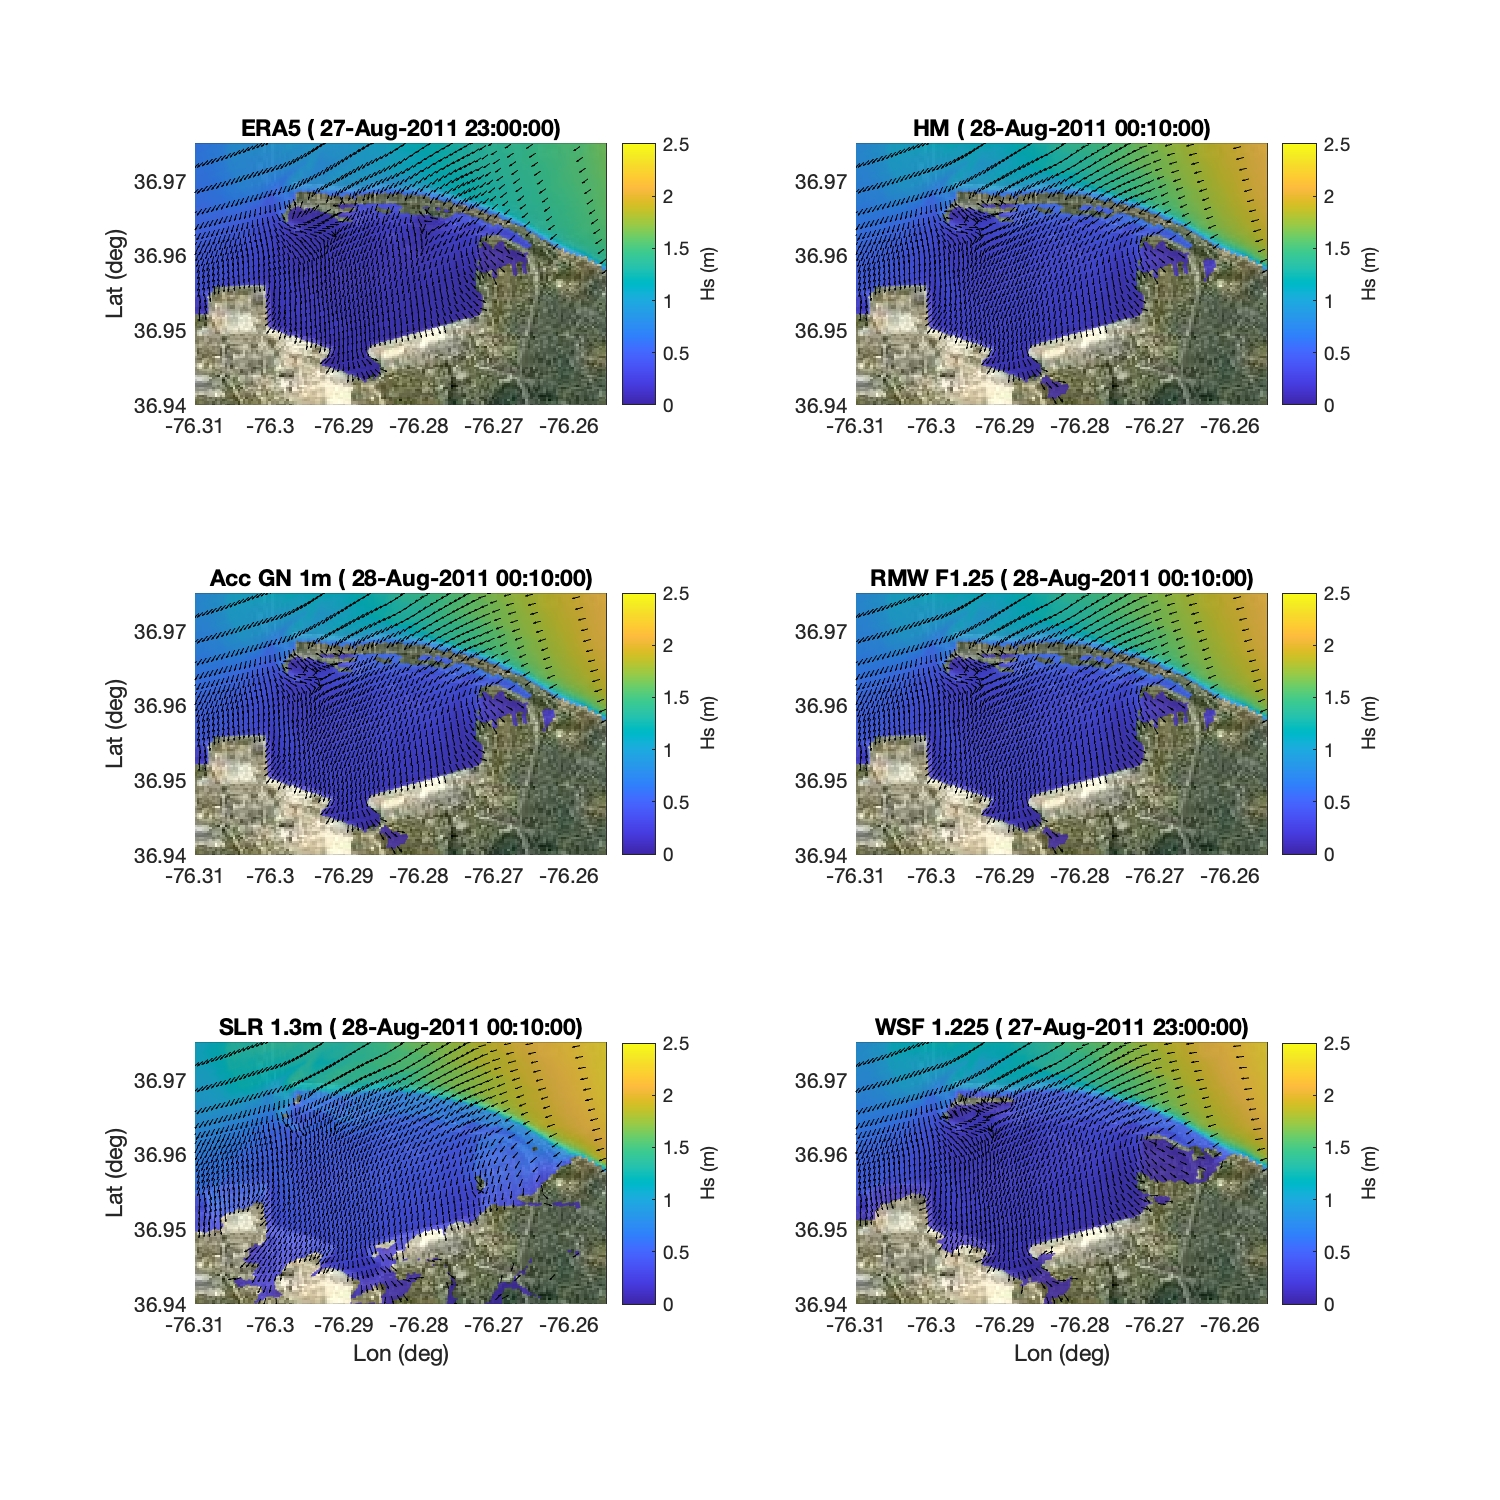
\includegraphics[width=\textwidth]{./figures/nearcom_hs.jpg}
\caption{NEARCOM results of significant wave height (color) and wave direction (vectors) at the peak storm tide from the six selected scenarios.}
\label{nearcom_6_cases_hs}
\centering
\end{figure}

\begin{figure}[h!]
\centering
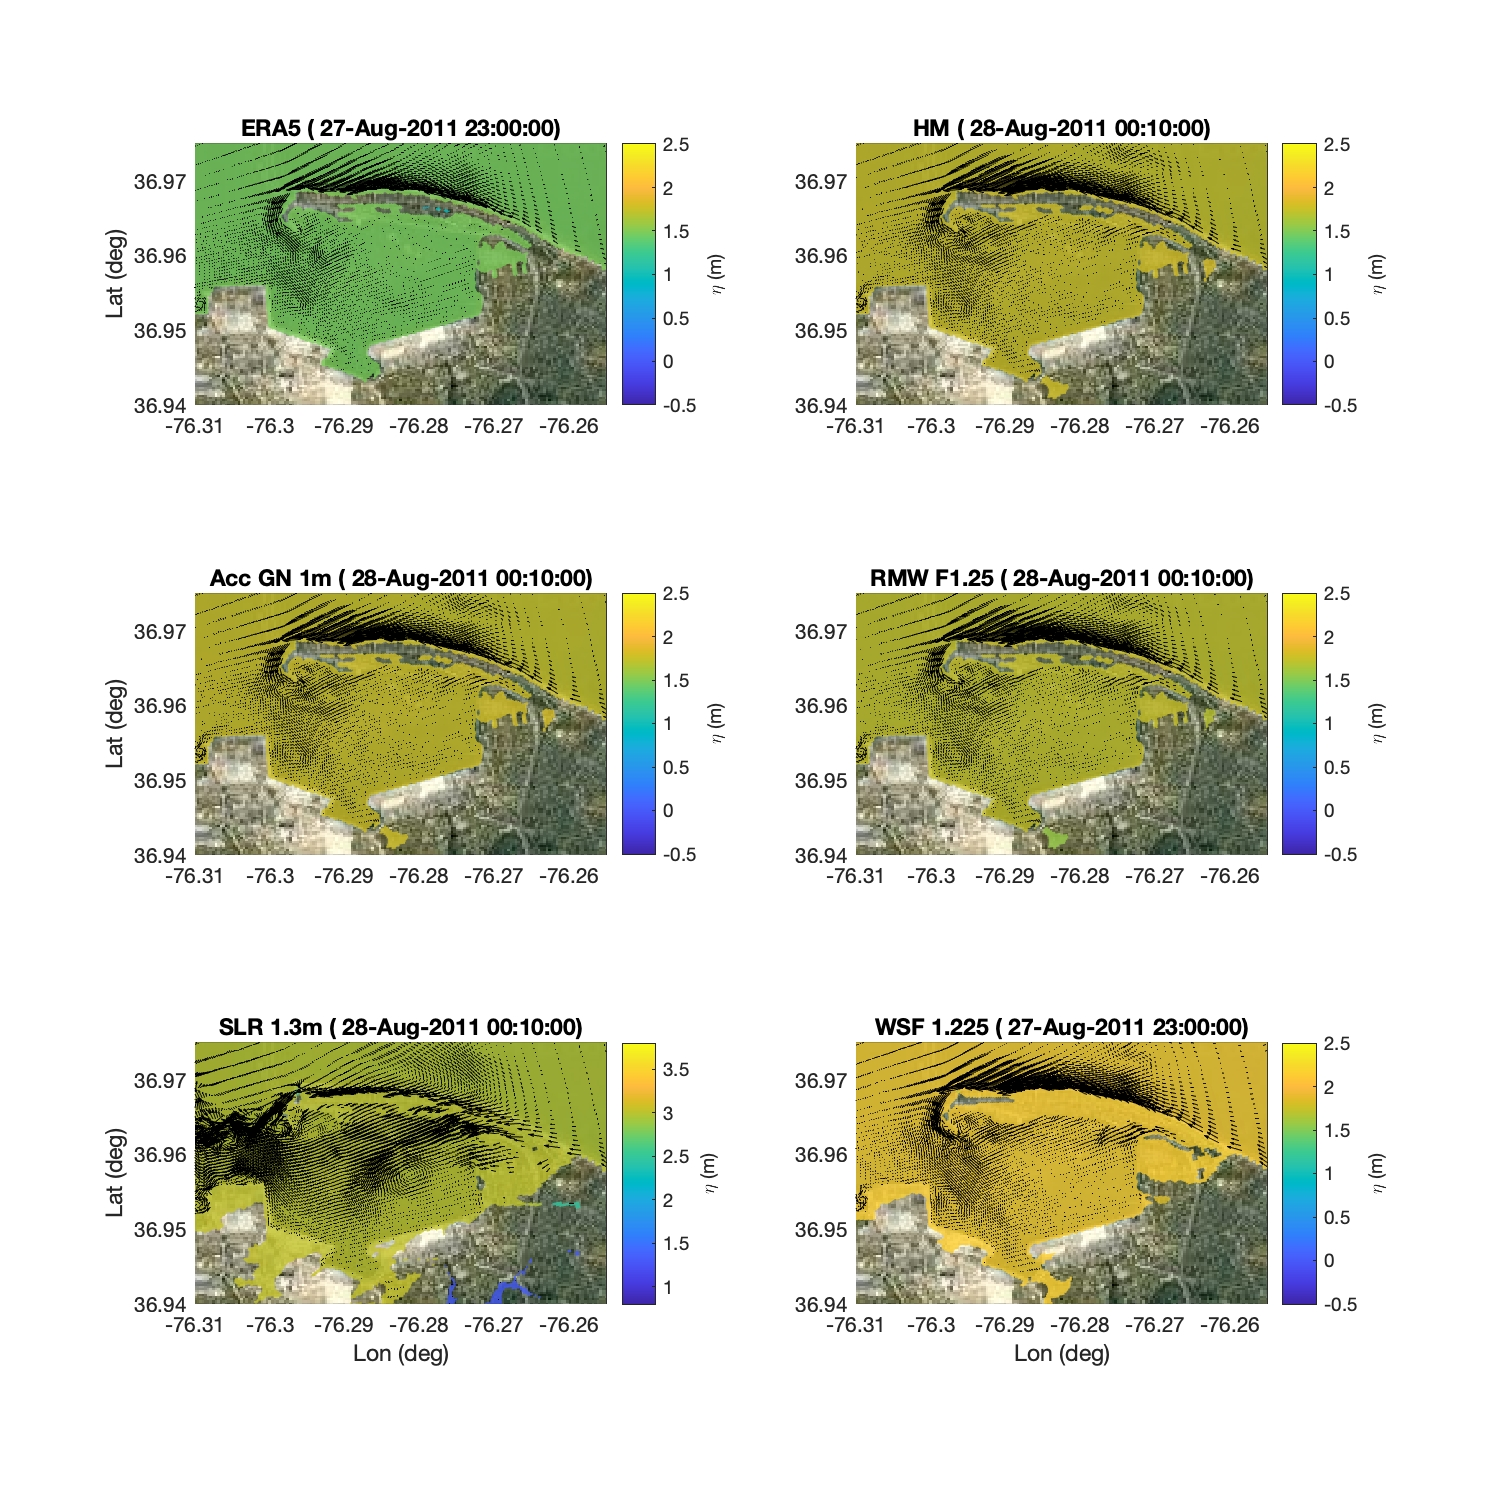
\includegraphics[width=\textwidth]{./figures/nearcom_eta_uv.jpg}
\caption{NEARCOM results of surface elevation (color) and currents (vectors) at the peak storm tide from the six selected scenarios}
\label{nearcom_6_cases_eta}
\centering
\end{figure}

\begin{figure}[h!]
\centering
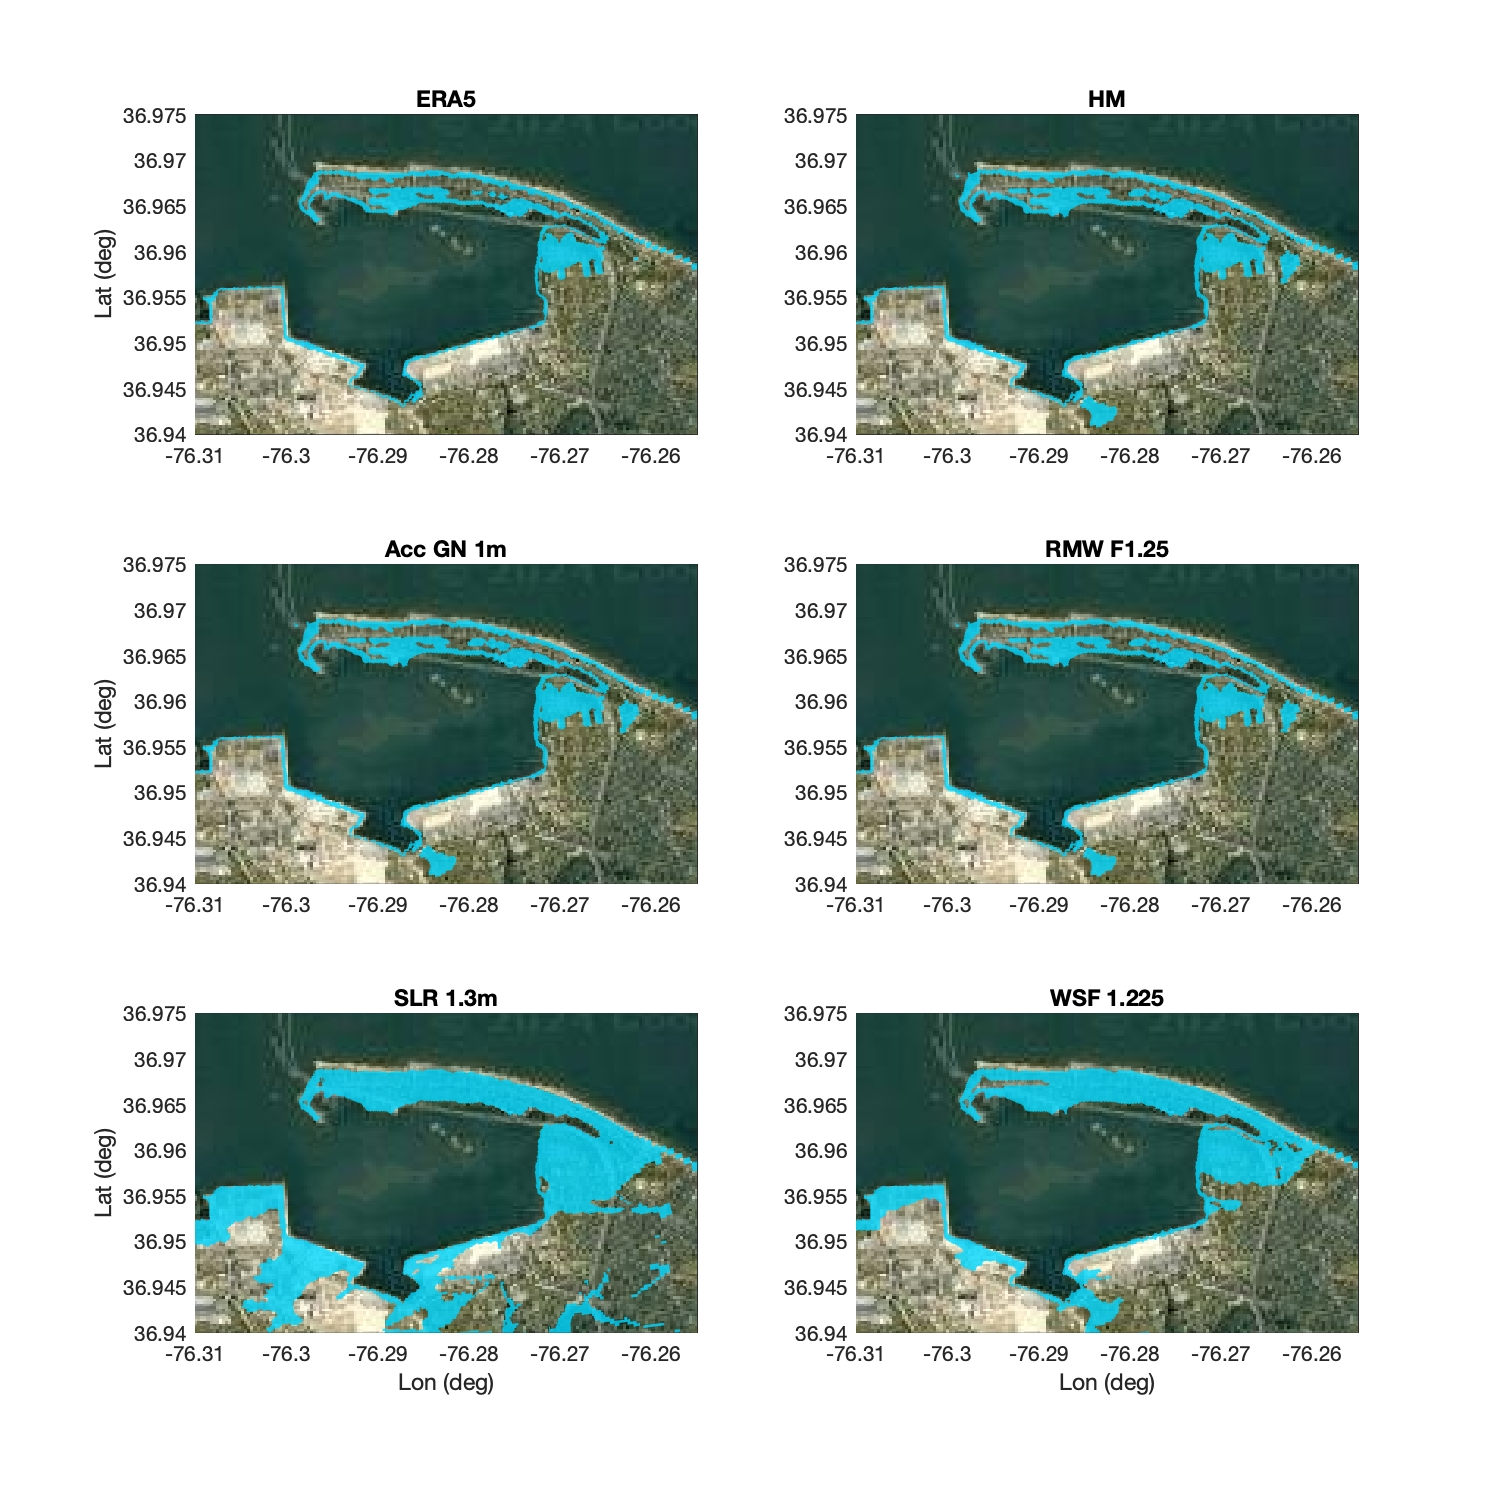
\includegraphics[width=\textwidth]{./figures/nearcom_flood.jpg}
\caption{NEARCOM results of flooded area (blue color) from the six selected scenarios.}
\label{nearcom_6_cases_flood}
\centering
\end{figure}

\begin{figure}[h!]
\centering
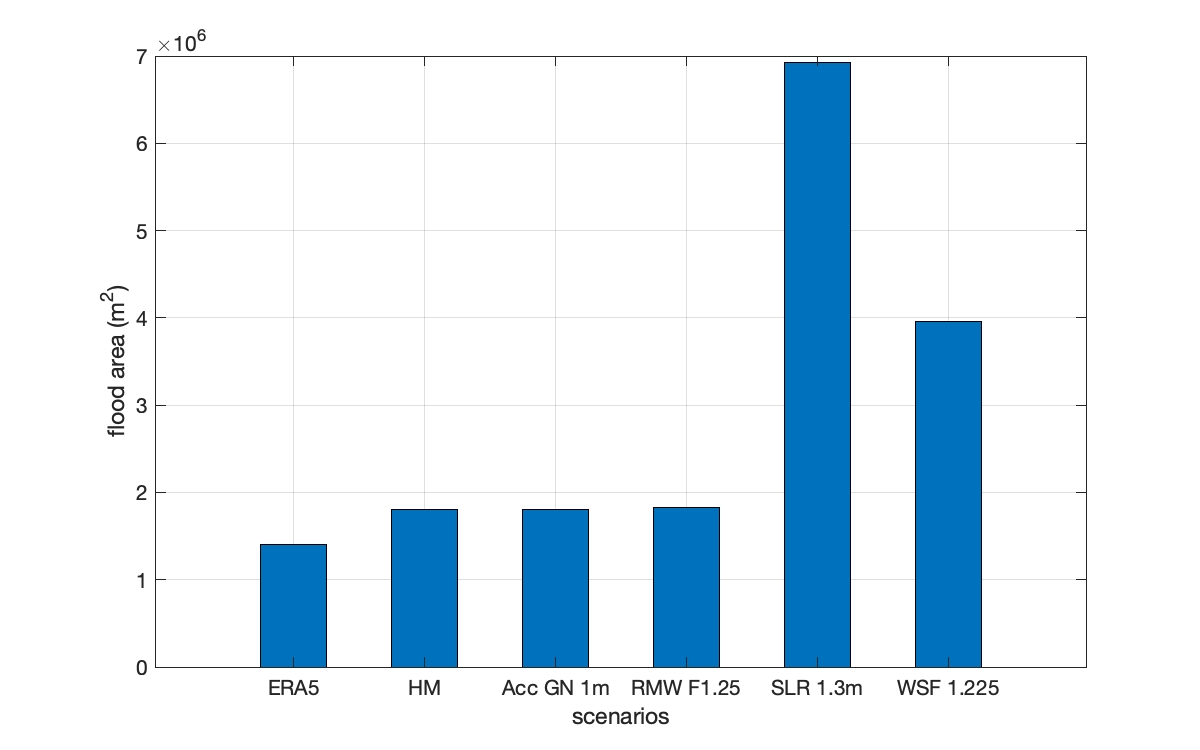
\includegraphics[width=\textwidth]{./figures/nearcom_bars.jpg}
\caption{Flooded areas (m$^2$) in the NEARCOM computational domain from the six selected scenarios.}
\label{nearcom_bars}
\centering
\end{figure}

% funwave

%\newpage
\section*{6.6 FUNWAVE}

Input wave conditions were from the SWAN simulation at the peak of the storm tide. 
Table X lists the wave conditions used in the six selected scenarios. Simulation time is one hour for each scenario. 

\begin{table}[h!]
 \caption{Wave conditions in the scenarios modeled by FUNWAVE-TVD}
 \centering
 \begin{tabular}[t]{c c c c  c c} \hline
  Scenario & Storm Tide (m) &Wave Height (m)  &  Wave Period (s)  &  Mean Direction (deg, Nautical) &  Direction Spreading (deg)  \\ \hline
  ERA5            &  1.55    & 1.78  & 5.99  & 60.5 & 38.0  \\
  HM                &   1.76   & 2.02  & 5.99  & 89.0 & 35.0  \\
  Acc GN 1m.   &   1.75  & 2.02  & 5.99  & 88.0 & 35.0  \\
  RMW F1.25   &    1.66 & 1.95  & 5.99  & 88.0 & 36.0  \\
   SLR 1.3m      &   3.02 & 2.35  & 6.81  & 88.0 & 35.0  \\
    WSF 1.225   &   2.45  & 2.31  & 5.99  & 98.8 & 33.0  \\
     \hline
 \end{tabular}
% \vskip 0.2cm
\end{table}


\begin{figure}[h!]
\centering
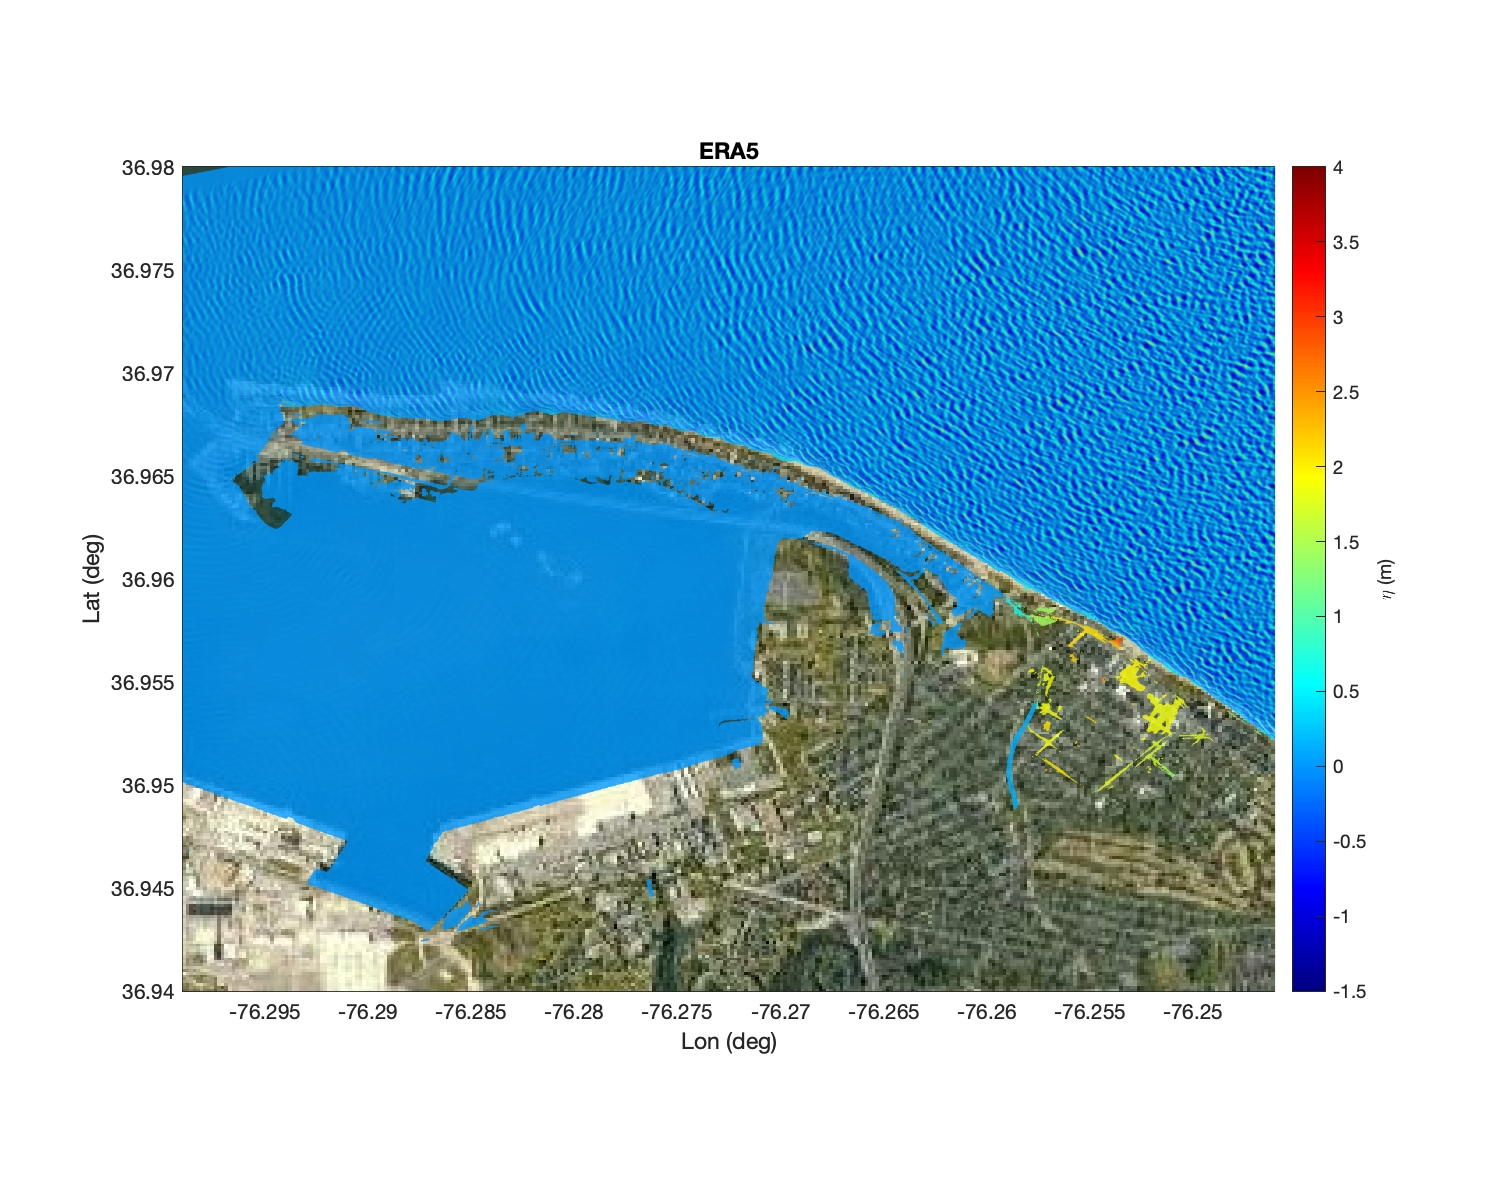
\includegraphics[width=\textwidth]{./figures/funwave_ERA5_eta.jpg}
\caption{Snapshot of wave surface at the peak of the storm tide (27-Aug-2011 23:00) modeled by FUNWAVE-TVD for scenario ERA5. }
\label{funwave_ERA5_eta}
\centering
\end{figure}

Figure \ref{funwave_ERA5_eta} shows a snapshot of wave field for Scenario ERA5. Waves on the east side of the domain appear to be more broadly spread compared to the west side, indicating the refraction effect due to the coastal bathymetry. Short waves do not appear inside Willoughby Bay.  The similar results for the wave field are obtained for other scenarios, except Scenario SLR 1.3m, which shows larger waves along the coast as depicted in Figure \ref{funwave_SLR_eta}. 

\begin{figure}[h!]
\centering
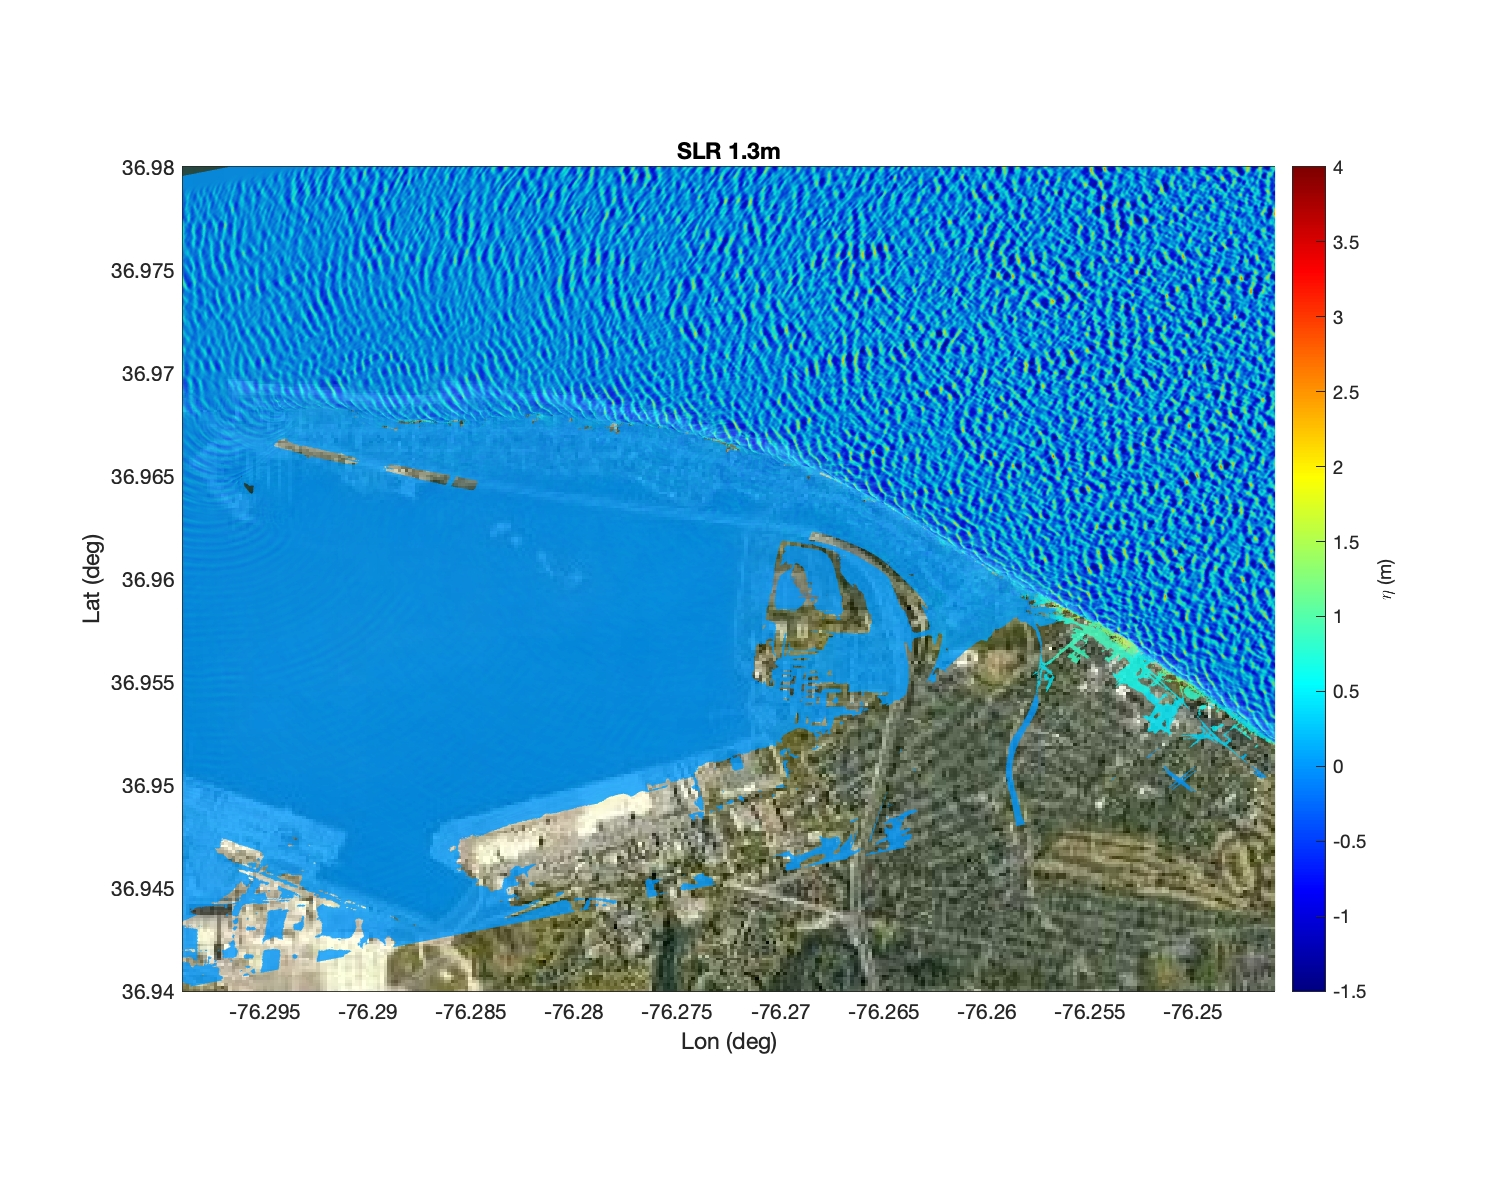
\includegraphics[width=\textwidth]{./figures/funwave_SLR _eta.jpg}
\caption{Snapshot of wave surface at the peak of the storm tide (27-Aug-2011 23:00) modeled by FUNWAVE-TVD for scenario SLR 1.3 m. }
\label{funwave_SLR_eta}
\centering
\end{figure}

\begin{figure}[h!]
\centering
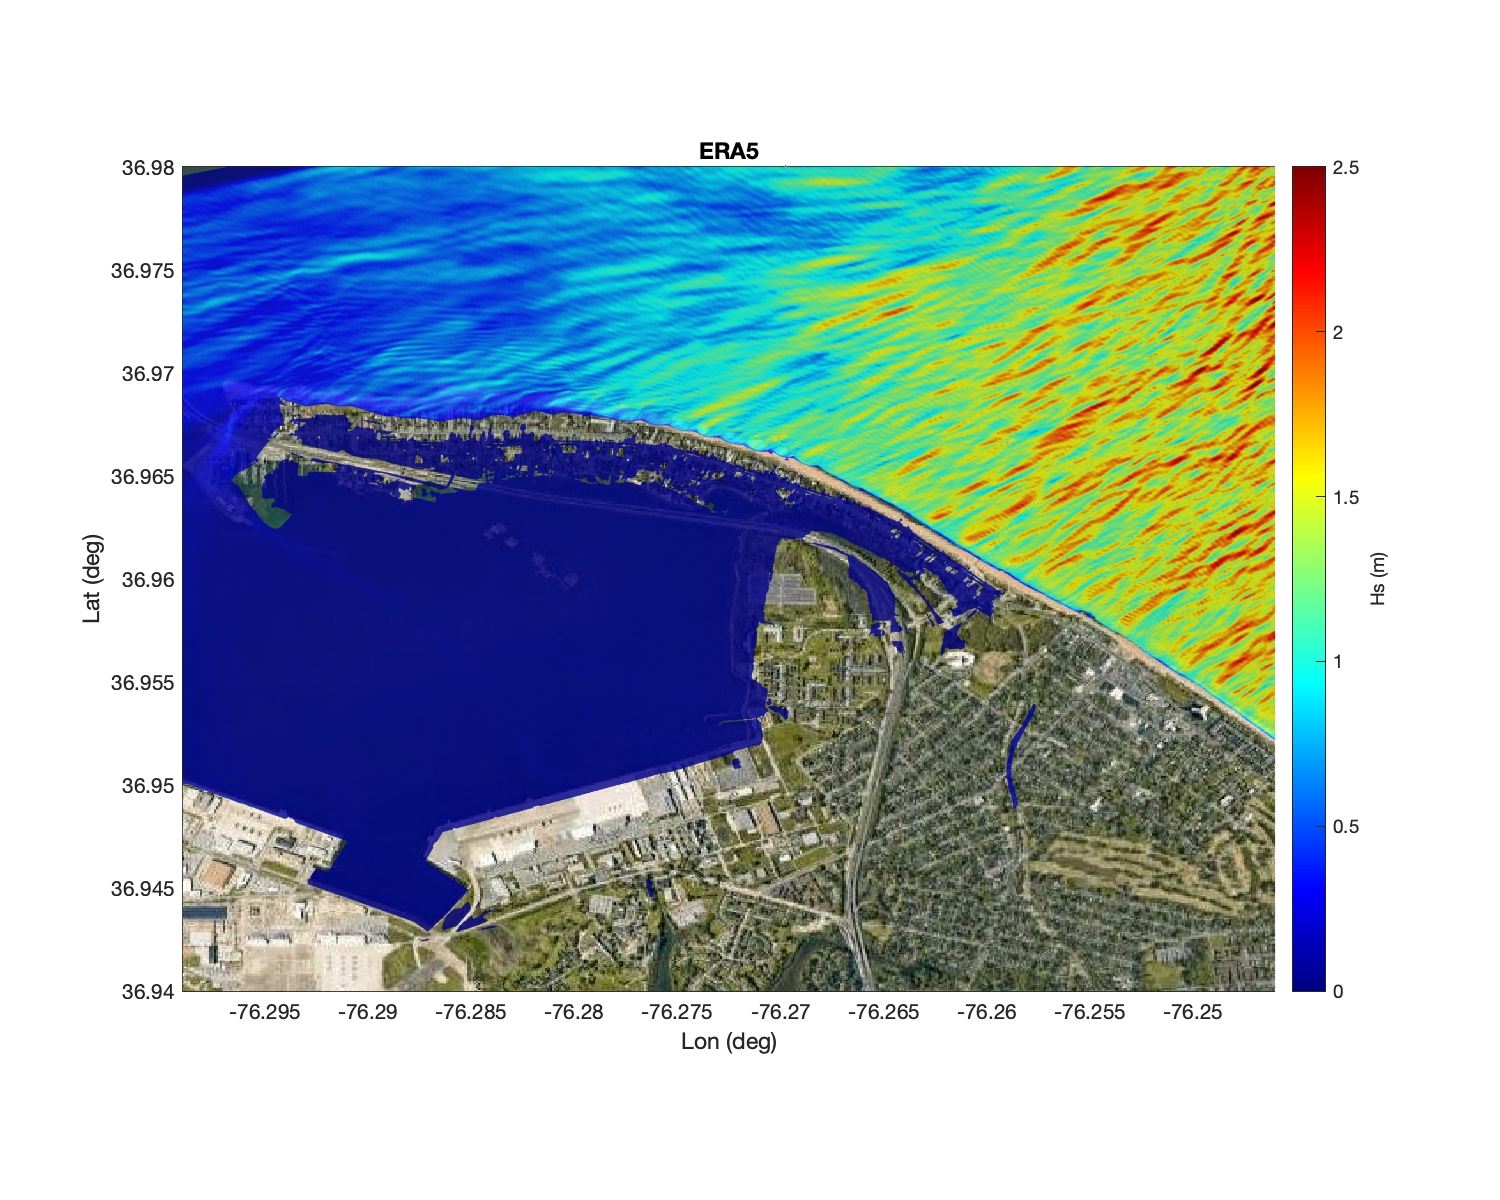
\includegraphics[width=\textwidth]{./figures/funwave_ERA5_hs.jpg}
\caption{FUNWAVE-TVD result of significant wave height at the peak storm tide (27-Aug-2011 23:00) for scenarios ERA5.  }
\label{funwave_ERA5_hs}
\centering
\end{figure}

The differences between Scenario SLR 1.3m and other cases is evident in wave height distribution as shown in Figures \ref{funwave_ERA5_hs} and \ref{funwave_SLR_hs}, which compare the significant wave heights between Scenarios ERA5 and SLR 1.3m. 

%The significant wave heights are calculated using 
%\be
%H_{sig} = 4.004 \frac{1}{t_2-t_1} \int_{t_1}^{t_2} \eta dt
%\ee

Although most of areas of Willoughby Split are flooded in Scenario SLR 1.3m, waves in the flooded areas are insignificant due to wave dissipation in the shallow water. 

\begin{figure}[h!]
\centering
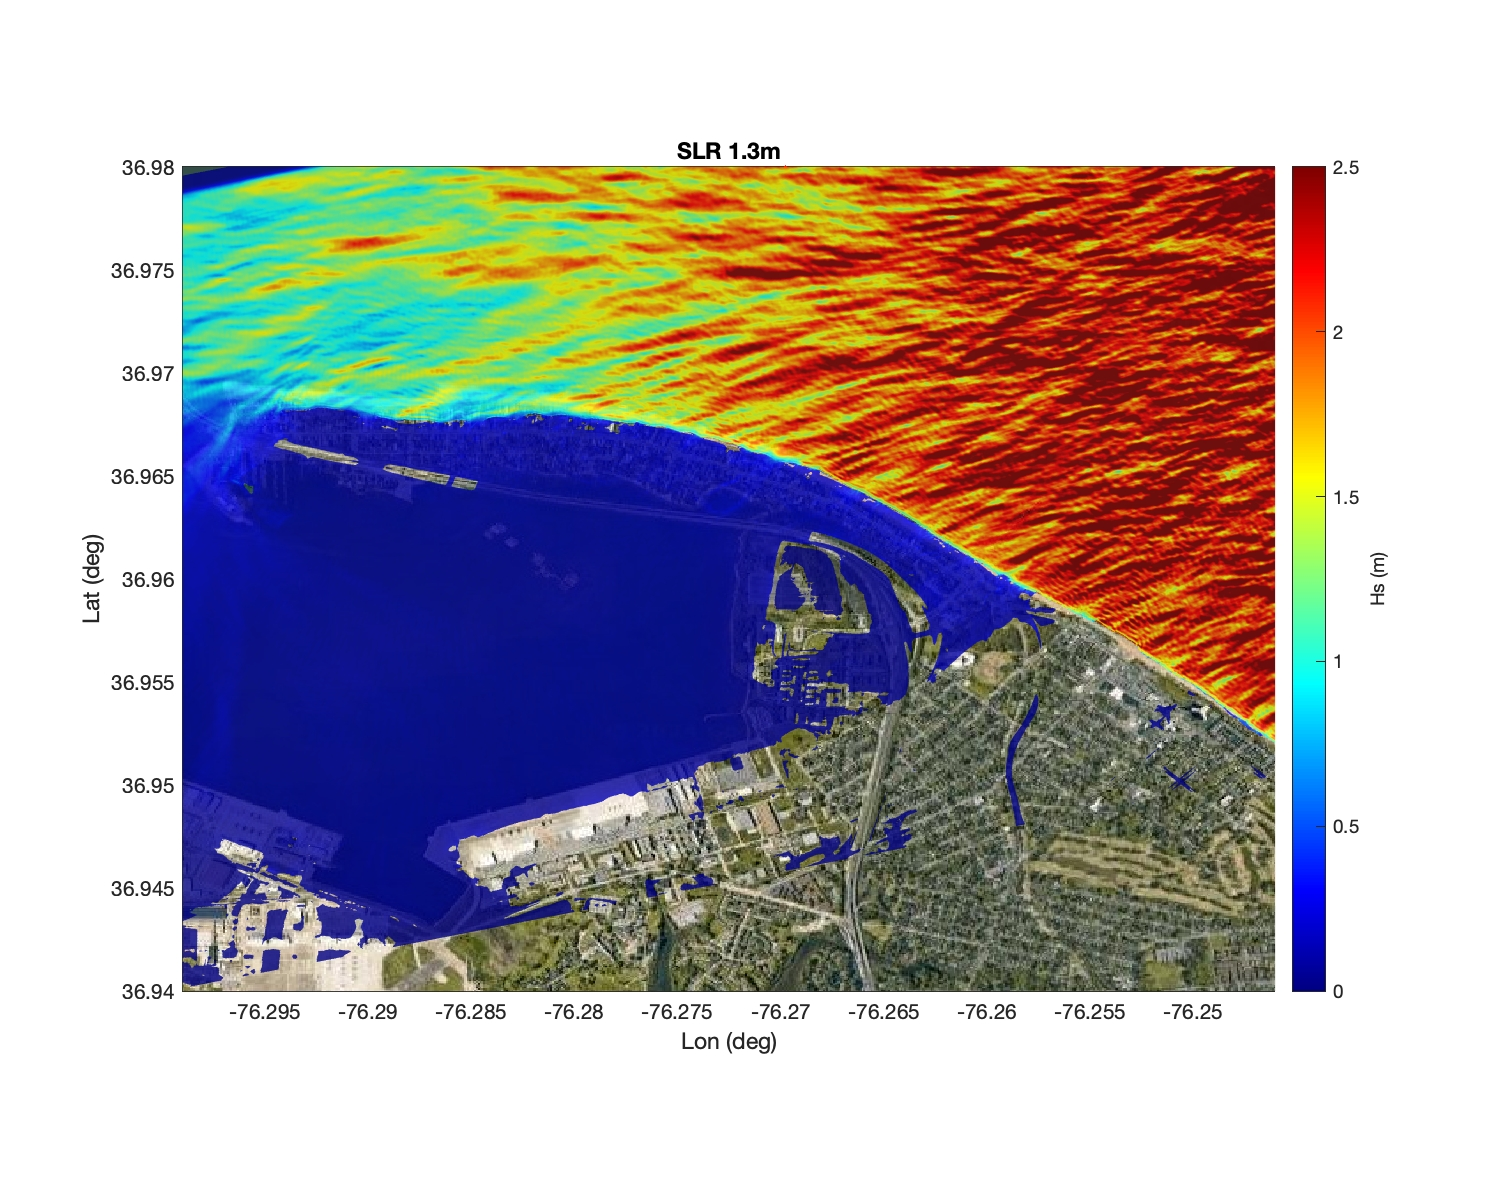
\includegraphics[width=\textwidth]{./figures/funwave_SLR_hs.jpg}
\caption{FUNWAVE-TVD result of significant wave height at the peak storm tide (27-Aug-2011 23:00) for scenarios SLR 1.3 m.  }
\label{funwave_SLR_hs}
\centering
\end{figure}

FUNWAVE-TVD can also predict wave setup by averaging the surface elevation over certain number of the peak wave period. Figure \ref{funwave_ERA5_setup} demonstrates wave setup for Scenario ERA5. Wave setup is primarily distributed in the surfzone along the coast, with a magnitude of 0.1m, consistent with the NEARCOM prediction. The surface elevation inside Willoughby Bay is not significantly affected much bye the wave setup at the coast.  

\begin{figure}[h!]
\centering
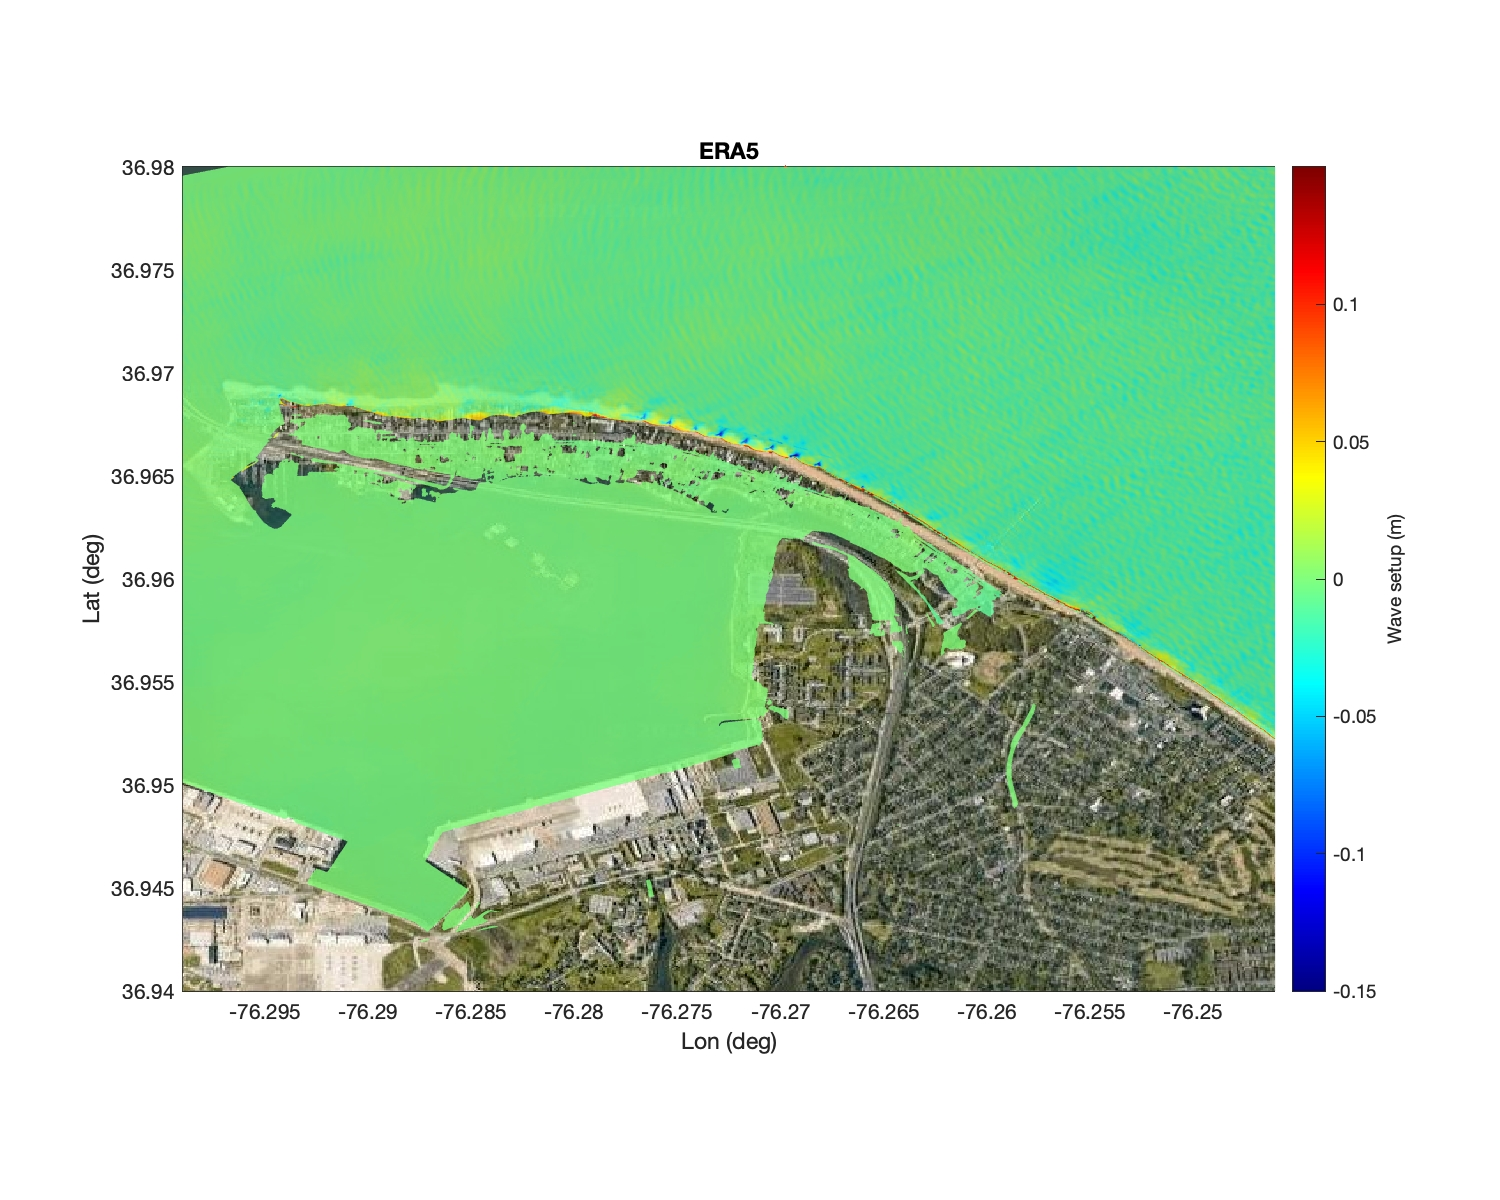
\includegraphics[width=\textwidth]{./figures/funwave_ERA5_setup.jpg}
\caption{FUNWAVE-TVD result of wave setup at the peak storm tide (27-Aug-2011 23:00) for scenarios ERA5.  }
\label{funwave_ERA5_setup}
\centering
\end{figure}

\begin{figure}[h!]
\centering
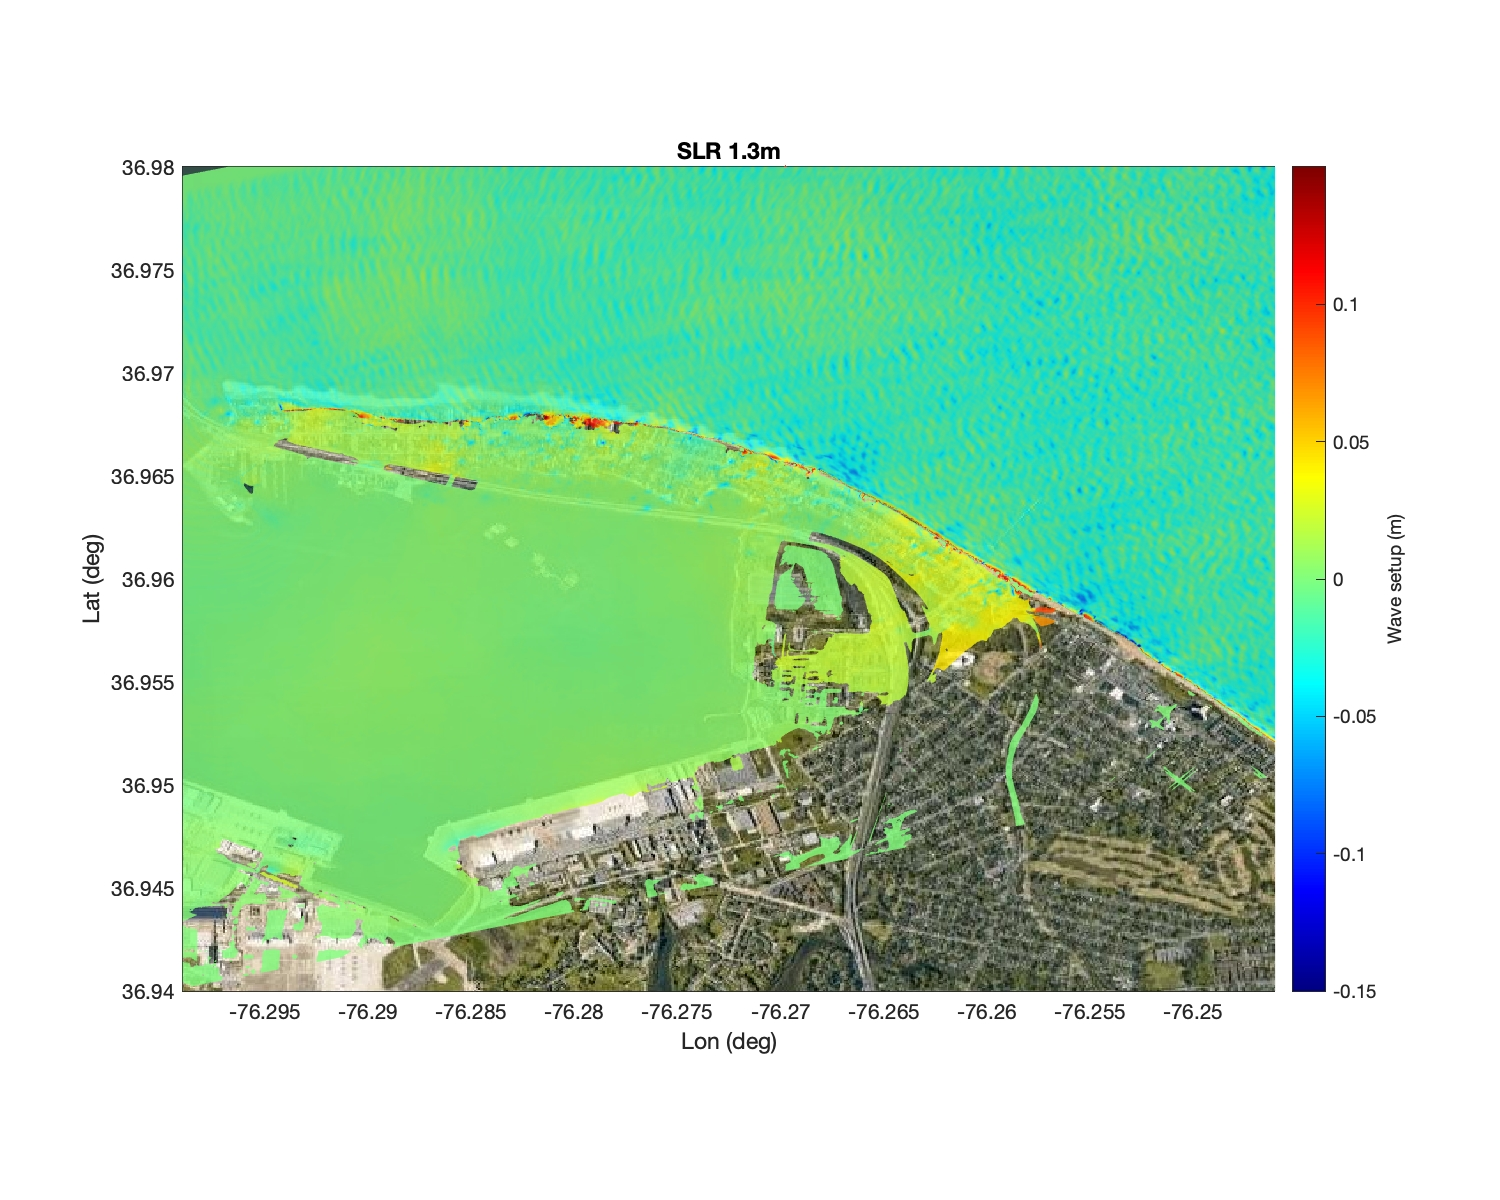
\includegraphics[width=\textwidth]{./figures/funwave_SLR_setup.jpg}
\caption{FUNWAVE-TVD result of wave setup at the peak storm tide (27-Aug-2011 23:00) for scenarios SLR 1.3 m. }
\label{funwave_SLR_setup}
\centering
\end{figure}

The distribution of wave-induced elevation for Scenario SLR 1.3m exhibits a different pattern as shown in Figure \ref{funwave_SLR_setup}. Inside Willoughby Bay, the surface elevation is significantly affected by waves due to wave setup, runup and overtopping. The wave distributions from the other four cases are similar, not shown here.  

\begin{figure}[h!]
\centering
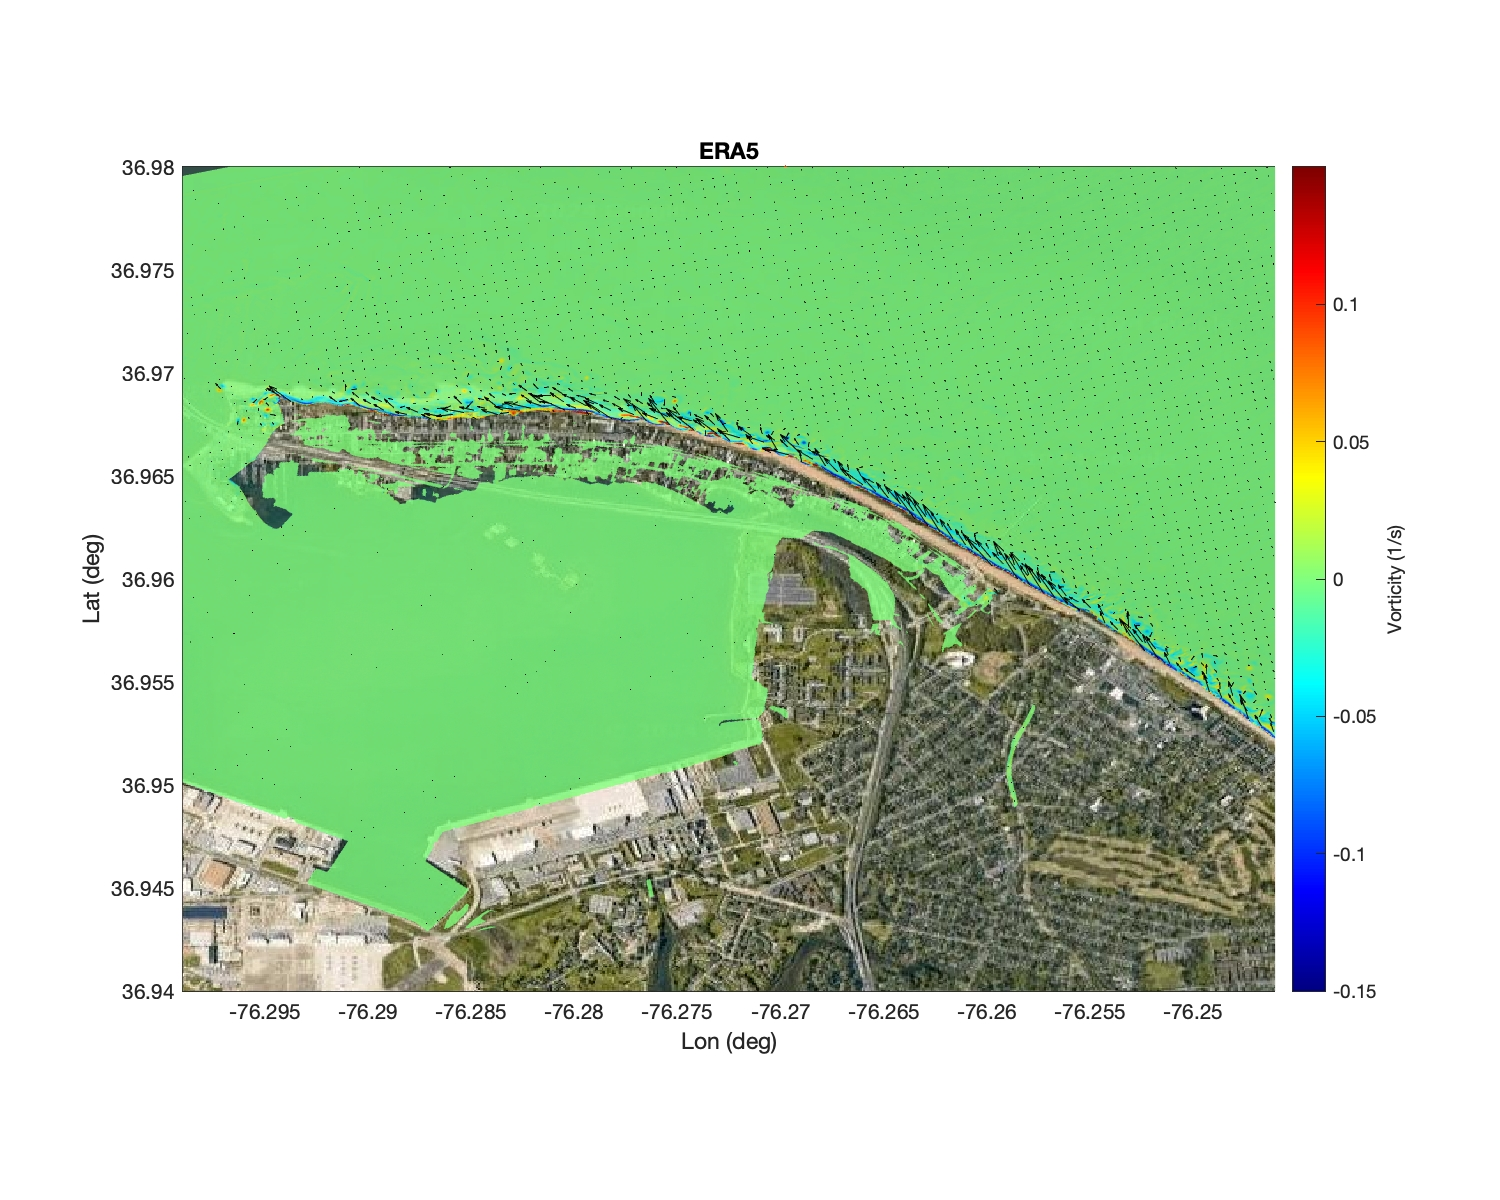
\includegraphics[width=\textwidth]{./figures/funwave_ERA5_vort.jpg}
\caption{FUNWAVE results of wave-induced current (vectors) and vertical vorticity (color) at the peak storm tide (27-Aug-2011 23:00) for scenarios ERA5. }
\label{funwave_ERA5_vort}
\centering
\end{figure}

\begin{figure}[h!]
\centering
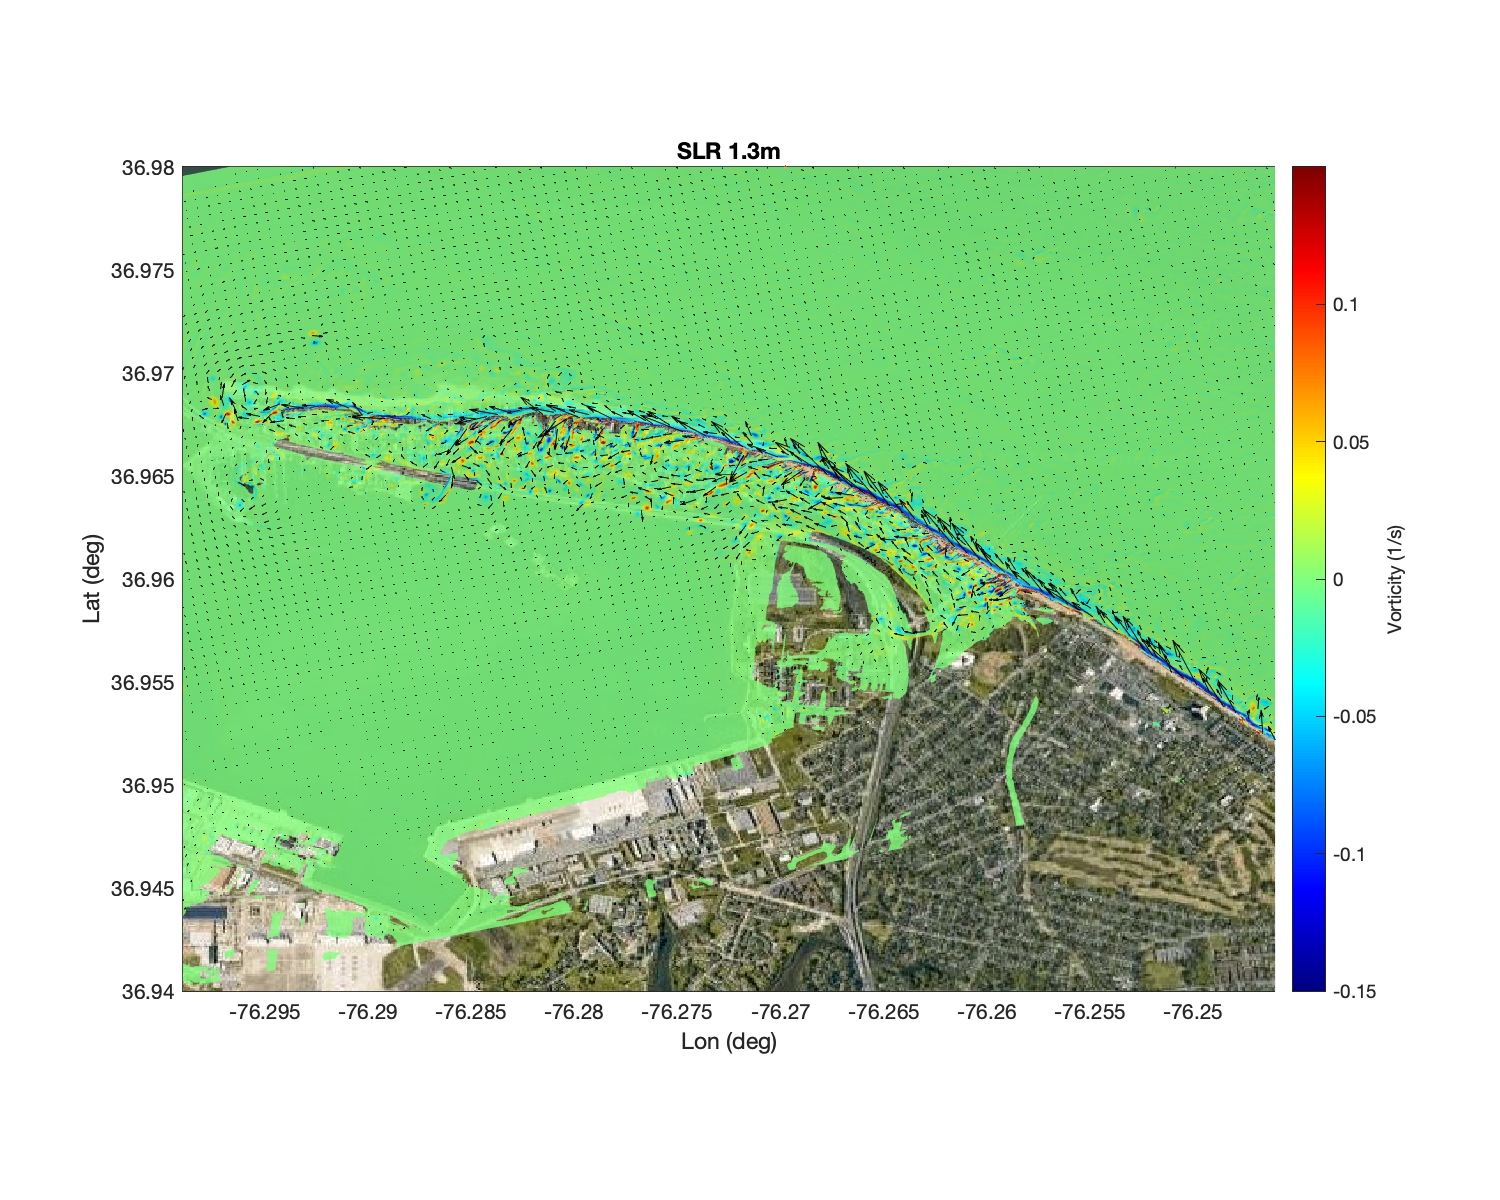
\includegraphics[width=\textwidth]{./figures/funwave_SLR_vort.jpg}
\caption{FUNWAVE results of wave-induced current (vectors) and vertical vorticity (color) at the peak storm tide (27-Aug-2011 23:00) for scenarios SLR 1.3 m.}
\label{funwave_SLR_vort}
\centering
\end{figure}

Wave-induced currents for Scenarios ERA5 and SLR 1.3m are shown in Figures \ref{funwave_ERA5_vort} and \ref{funwave_SLR_vort}, respectively. Colors represent vertical vorticity associated with the currents. In Scenario ERA5, the wave-induced current are concentrates in the surfzone alongshore the Willoughby Spit coast, consistent with the NEAECOM results. However, the surfzone predicted by FUNWAVE-TVD appear  narrower, likely due to the higher grid resolution used in the model. For Scenario SLR 1.3m, wave-induced currents are more complex due to the flooding of Willoughby Split. Eddies are generated in the flooded areas. 



\begin{figure}[h!]
\centering
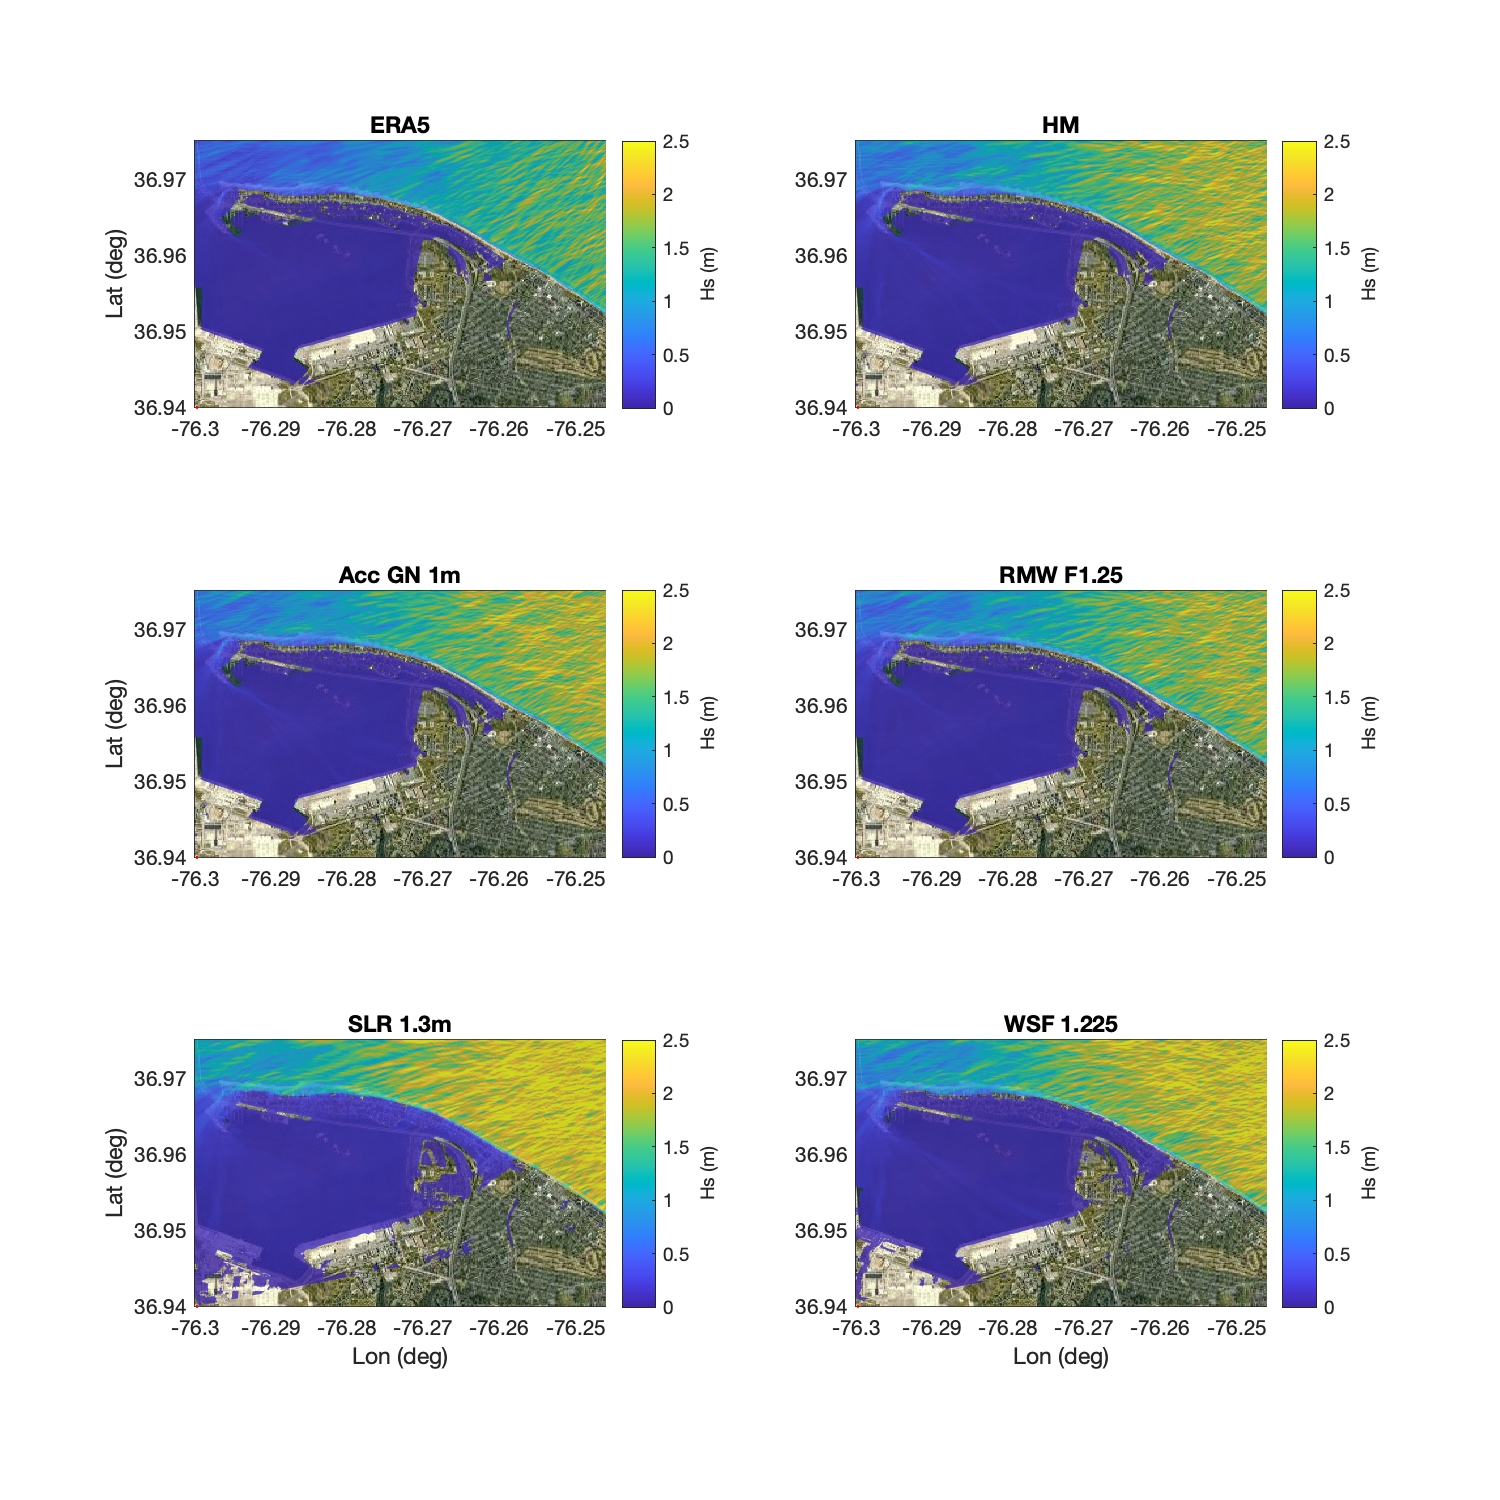
\includegraphics[width=\textwidth]{./figures/funwave_hs_6_cases.jpg}
\caption{FUNWAVE-TVD results of significant wave height  at the peak storm tide from the six selected scenarios. }
\label{funwave_6_cases_hs}
\centering
\end{figure}

Wave height distributions from all six cases are compared in Figure \ref{funwave_6_cases_hs}. The results are consistent with the NEARCOM results. 

\end{document}